% Created 2022-04-17 Sun 14:58
% Intended LaTeX compiler: pdflatex
\documentclass[11pt]{article}
\usepackage[utf8]{inputenc}
\usepackage[T1]{fontenc}
\usepackage{graphicx}
\usepackage{longtable}
\usepackage{wrapfig}
\usepackage{rotating}
\usepackage[normalem]{ulem}
\usepackage{amsmath}
\usepackage{amssymb}
\usepackage{capt-of}
\usepackage{hyperref}
\graphicspath{{../../books/}}
% wrong resolution of image
% https://tex.stackexchange.com/questions/21627/image-from-includegraphics-showing-in-wrong-image-size?rq=1

%%%%%%%%%%%%%%%%%%%%%%%%%%%%%%%%%%%%%%
%% TIPS                                 %%
%%%%%%%%%%%%%%%%%%%%%%%%%%%%%%%%%%%%%%
% \substack{a\\b} for multiple lines text
% \usepackage{expl3}
% \expandafter\def\csname ver@l3regex.sty\endcsname{}
% \usepackage{pkgloader}
\usepackage[utf8]{inputenc}

% nfss error
% \usepackage[B1,T1]{fontenc}
\usepackage{fontspec}

% \usepackage[Emoticons]{ucharclasses}
\newfontfamily\DejaSans{DejaVu Sans}
% \setDefaultTransitions{\DejaSans}{}

% pdfplots will load xolor automatically without option
\usepackage[dvipsnames]{xcolor}

%                                                             ┳┳┓   ┓
%                                                             ┃┃┃┏┓╋┣┓
%                                                             ┛ ┗┗┻┗┛┗
% \usepackage{amsmath} mathtools loads the amsmath
\usepackage{amsmath}
\usepackage{mathtools}

\usepackage{amsthm}
\usepackage{amsbsy}

%\usepackage{commath}

\usepackage{amssymb}

\usepackage{mathrsfs}
%\usepackage{mathabx}
\usepackage{stmaryrd}
\usepackage{empheq}

\usepackage{scalerel}
\usepackage{stackengine}
\usepackage{stackrel}



\usepackage{nicematrix}
\usepackage{tensor}
\usepackage{blkarray}
\usepackage{siunitx}
\usepackage[f]{esvect}

% centering \not on a letter
\usepackage{slashed}
\usepackage[makeroom]{cancel}

%\usepackage{merriweather}
\usepackage{unicode-math}
\setmainfont{TeX Gyre Pagella}
% \setmathfont{STIX}
%\setmathfont{texgyrepagella-math.otf}
%\setmathfont{Libertinus Math}
\setmathfont{Latin Modern Math}

 % \setmathfont[range={\smwhtdiamond,\enclosediamond,\varlrtriangle}]{Latin Modern Math}
\setmathfont[range={\rightrightarrows,\twoheadrightarrow,\leftrightsquigarrow,\triangledown,\vartriangle,\precneq,\succneq,\prec,\succ,\preceq,\succeq,\tieconcat}]{XITS Math}
 \setmathfont[range={\int,\setminus}]{Libertinus Math}
 % \setmathfont[range={\mathalpha}]{TeX Gyre Pagella Math}
%\setmathfont[range={\mitA,\mitB,\mitC,\mitD,\mitE,\mitF,\mitG,\mitH,\mitI,\mitJ,\mitK,\mitL,\mitM,\mitN,\mitO,\mitP,\mitQ,\mitR,\mitS,\mitT,\mitU,\mitV,\mitW,\mitX,\mitY,\mitZ,\mita,\mitb,\mitc,\mitd,\mite,\mitf,\mitg,\miti,\mitj,\mitk,\mitl,\mitm,\mitn,\mito,\mitp,\mitq,\mitr,\mits,\mitt,\mitu,\mitv,\mitw,\mitx,\mity,\mitz}]{TeX Gyre Pagella Math}
% unicode is not good at this!
%\let\nmodels\nvDash

 \usepackage{wasysym}

 % for wide hat
 \DeclareSymbolFont{yhlargesymbols}{OMX}{yhex}{m}{n} \DeclareMathAccent{\what}{\mathord}{yhlargesymbols}{"62}

%                                                               ┏┳┓•┓
%                                                                ┃ ┓┃┏┓
%                                                                ┻ ┗┛┗┗

\usepackage{pgfplots}
\pgfplotsset{compat=1.18}
\usepackage{tikz}
\usepackage{tikz-cd}
\tikzcdset{scale cd/.style={every label/.append style={scale=#1},
    cells={nodes={scale=#1}}}}
% TODO: discard qtree and use forest
% \usepackage{tikz-qtree}
\usepackage{forest}

\usetikzlibrary{arrows,positioning,calc,fadings,decorations,matrix,decorations,shapes.misc}
%setting from geogebra
\definecolor{ccqqqq}{rgb}{0.8,0,0}

%                                                          ┳┳┓•    ┓┓
%                                                          ┃┃┃┓┏┏┏┓┃┃┏┓┏┓┏┓┏┓┓┏┏
%                                                          ┛ ┗┗┛┗┗ ┗┗┗┻┛┗┗ ┗┛┗┻┛
%\usepackage{twemojis}
\usepackage[most]{tcolorbox}
\usepackage{threeparttable}
\usepackage{tabularx}

\usepackage{enumitem}
\usepackage[indLines=false]{algpseudocodex}
\usepackage[]{algorithm2e}
% \SetKwComment{Comment}{/* }{ */}
% \algrenewcommand\algorithmicrequire{\textbf{Input:}}
% \algrenewcommand\algorithmicensure{\textbf{Output:}}
% wrong with preview
\usepackage{subcaption}
\usepackage{caption}
% {\aunclfamily\Huge}
\usepackage{auncial}

\usepackage{float}

\usepackage{fancyhdr}

\usepackage{ifthen}
\usepackage{xargs}

\definecolor{mintedbg}{rgb}{0.99,0.99,0.99}
\usepackage[cachedir=\detokenize{~/miscellaneous/trash}]{minted}
\setminted{breaklines,
  mathescape,
  bgcolor=mintedbg,
  fontsize=\footnotesize,
  frame=single,
  linenos}
\usemintedstyle{xcode}
\usepackage{tcolorbox}
\usepackage{etoolbox}



\usepackage{imakeidx}
\usepackage{hyperref}
\usepackage{soul}
\usepackage{framed}

% don't use this for preview
%\usepackage[margin=1.5in]{geometry}
% \usepackage{geometry}
% \geometry{legalpaper, landscape, margin=1in}
\usepackage[font=itshape]{quoting}

%\LoadPackagesNow
%\usepackage[xetex]{preview}
%%%%%%%%%%%%%%%%%%%%%%%%%%%%%%%%%%%%%%%
%% USEPACKAGES end                       %%
%%%%%%%%%%%%%%%%%%%%%%%%%%%%%%%%%%%%%%%

%%%%%%%%%%%%%%%%%%%%%%%%%%%%%%%%%%%%%%%
%% Algorithm environment
%%%%%%%%%%%%%%%%%%%%%%%%%%%%%%%%%%%%%%%
\SetKwIF{Recv}{}{}{upon receiving}{do}{}{}{}
\SetKwBlock{Init}{initially do}{}
\SetKwProg{Function}{Function}{:}{}

% https://github.com/chrmatt/algpseudocodex/issues/3
\algnewcommand\algorithmicswitch{\textbf{switch}}%
\algnewcommand\algorithmiccase{\textbf{case}}
\algnewcommand\algorithmicof{\textbf{of}}
\algnewcommand\algorithmicotherwise{\texttt{otherwise} $\Rightarrow$}

\makeatletter
\algdef{SE}[SWITCH]{Switch}{EndSwitch}[1]{\algpx@startIndent\algpx@startCodeCommand\algorithmicswitch\ #1\ \algorithmicdo}{\algpx@endIndent\algpx@startCodeCommand\algorithmicend\ \algorithmicswitch}%
\algdef{SE}[CASE]{Case}{EndCase}[1]{\algpx@startIndent\algpx@startCodeCommand\algorithmiccase\ #1}{\algpx@endIndent\algpx@startCodeCommand\algorithmicend\ \algorithmiccase}%
\algdef{SE}[CASEOF]{CaseOf}{EndCaseOf}[1]{\algpx@startIndent\algpx@startCodeCommand\algorithmiccase\ #1 \algorithmicof}{\algpx@endIndent\algpx@startCodeCommand\algorithmicend\ \algorithmiccase}
\algdef{SE}[OTHERWISE]{Otherwise}{EndOtherwise}[0]{\algpx@startIndent\algpx@startCodeCommand\algorithmicotherwise}{\algpx@endIndent\algpx@startCodeCommand\algorithmicend\ \algorithmicotherwise}
\ifbool{algpx@noEnd}{%
  \algtext*{EndSwitch}%
  \algtext*{EndCase}%
  \algtext*{EndCaseOf}
  \algtext*{EndOtherwise}
  %
  % end indent line after (not before), to get correct y position for multiline text in last command
  \apptocmd{\EndSwitch}{\algpx@endIndent}{}{}%
  \apptocmd{\EndCase}{\algpx@endIndent}{}{}%
  \apptocmd{\EndCaseOf}{\algpx@endIndent}{}{}
  \apptocmd{\EndOtherwise}{\algpx@endIndent}{}{}
}{}%

\pretocmd{\Switch}{\algpx@endCodeCommand}{}{}
\pretocmd{\Case}{\algpx@endCodeCommand}{}{}
\pretocmd{\CaseOf}{\algpx@endCodeCommand}{}{}
\pretocmd{\Otherwise}{\algpx@endCodeCommand}{}{}

% for end commands that may not be printed, tell endCodeCommand whether we are using noEnd
\ifbool{algpx@noEnd}{%
  \pretocmd{\EndSwitch}{\algpx@endCodeCommand[1]}{}{}%
  \pretocmd{\EndCase}{\algpx@endCodeCommand[1]}{}{}
  \pretocmd{\EndCaseOf}{\algpx@endCodeCommand[1]}{}{}%
  \pretocmd{\EndOtherwise}{\algpx@endCodeCommand[1]}{}{}
}{%
  \pretocmd{\EndSwitch}{\algpx@endCodeCommand[0]}{}{}%
  \pretocmd{\EndCase}{\algpx@endCodeCommand[0]}{}{}%
  \pretocmd{\EndCaseOf}{\algpx@endCodeCommand[0]}{}{}
  \pretocmd{\EndOtherwise}{\algpx@endCodeCommand[0]}{}{}
}%
\makeatother
% % For algpseudocode
% \algnewcommand\algorithmicswitch{\textbf{switch}}
% \algnewcommand\algorithmiccase{\textbf{case}}
% \algnewcommand\algorithmiccaseof{\textbf{case}}
% \algnewcommand\algorithmicof{\textbf{of}}
% % New "environments"
% \algdef{SE}[SWITCH]{Switch}{EndSwitch}[1]{\algorithmicswitch\ #1\ \algorithmicdo}{\algorithmicend\ \algorithmicswitch}%
% \algdef{SE}[CASE]{Case}{EndCase}[1]{\algorithmiccase\ #1}{\algorithmicend\ \algorithmiccase}%
% \algtext*{EndSwitch}%
% \algtext*{EndCase}
% \algdef{SE}[CASEOF]{CaseOf}{EndCaseOf}[1]{\algorithmiccaseof\ #1 \algorithmicof}{\algorithmicend\ \algorithmiccaseof}
% \algtext*{EndCaseOf}



%\pdfcompresslevel0

% quoting from
% https://tex.stackexchange.com/questions/391726/the-quotation-environment
\NewDocumentCommand{\bywhom}{m}{% the Bourbaki trick
  {\nobreak\hfill\penalty50\hskip1em\null\nobreak
   \hfill\mbox{\normalfont(#1)}%
   \parfillskip=0pt \finalhyphendemerits=0 \par}%
}

\NewDocumentEnvironment{pquotation}{m}
  {\begin{quoting}[
     indentfirst=true,
     leftmargin=\parindent,
     rightmargin=\parindent]\itshape}
  {\bywhom{#1}\end{quoting}}

\indexsetup{othercode=\small}
\makeindex[columns=2,options={-s /media/wu/file/stuuudy/notes/index_style.ist},intoc]
\makeatletter
\def\@idxitem{\par\hangindent 0pt}
\makeatother


% \newcounter{dummy} \numberwithin{dummy}{section}
\newtheorem{dummy}{dummy}[section]
\theoremstyle{definition}
\newtheorem{definition}[dummy]{Definition}
\theoremstyle{plain}
\newtheorem{corollary}[dummy]{Corollary}
\newtheorem{lemma}[dummy]{Lemma}
\newtheorem{proposition}[dummy]{Proposition}
\newtheorem{theorem}[dummy]{Theorem}
\newtheorem{notation}[dummy]{Notation}
\newtheorem{conjecture}[dummy]{Conjecture}
\newtheorem{fact}[dummy]{Fact}
\newtheorem{warning}[dummy]{Warning}
\theoremstyle{definition}
\newtheorem{examplle}{Example}[section]
\theoremstyle{remark}
\newtheorem*{remark}{Remark}
\newtheorem{exercise}{Exercise}[subsection]
\newtheorem{problem}{Problem}[subsection]
\newtheorem{observation}{Observation}[section]
\newenvironment{claim}[1]{\par\noindent\textbf{Claim:}\space#1}{}

\makeatletter
\DeclareFontFamily{U}{tipa}{}
\DeclareFontShape{U}{tipa}{m}{n}{<->tipa10}{}
\newcommand{\arc@char}{{\usefont{U}{tipa}{m}{n}\symbol{62}}}%

\newcommand{\arc}[1]{\mathpalette\arc@arc{#1}}

\newcommand{\arc@arc}[2]{%
  \sbox0{$\m@th#1#2$}%
  \vbox{
    \hbox{\resizebox{\wd0}{\height}{\arc@char}}
    \nointerlineskip
    \box0
  }%
}
\makeatother

\setcounter{MaxMatrixCols}{20}
%%%%%%% ABS
\DeclarePairedDelimiter\abss{\lvert}{\rvert}%
\DeclarePairedDelimiter\normm{\lVert}{\rVert}%

% Swap the definition of \abs* and \norm*, so that \abs
% and \norm resizes the size of the brackets, and the
% starred version does not.
\makeatletter
\let\oldabs\abss
%\def\abs{\@ifstar{\oldabs}{\oldabs*}}
\newcommand{\abs}{\@ifstar{\oldabs}{\oldabs*}}
\newcommand{\norm}[1]{\left\lVert#1\right\rVert}
%\let\oldnorm\normm
%\def\norm{\@ifstar{\oldnorm}{\oldnorm*}}
%\renewcommand{norm}{\@ifstar{\oldnorm}{\oldnorm*}}
\makeatother

% \stackMath
% \newcommand\what[1]{%
% \savestack{\tmpbox}{\stretchto{%
%   \scaleto{%
%     \scalerel*[\widthof{\ensuremath{#1}}]{\kern-.6pt\bigwedge\kern-.6pt}%
%     {\rule[-\textheight/2]{1ex}{\textheight}}%WIDTH-LIMITED BIG WEDGE
%   }{\textheight}%
% }{0.5ex}}%
% \stackon[1pt]{#1}{\tmpbox}%
% }

% \newcommand\what[1]{\ThisStyle{%
%     \setbox0=\hbox{$\SavedStyle#1$}%
%     \stackengine{-1.0\ht0+.5pt}{$\SavedStyle#1$}{%
%       \stretchto{\scaleto{\SavedStyle\mkern.15mu\char'136}{2.6\wd0}}{1.4\ht0}%
%     }{O}{c}{F}{T}{S}%
%   }
% }

% \newcommand\wtilde[1]{\ThisStyle{%
%     \setbox0=\hbox{$\SavedStyle#1$}%
%     \stackengine{-.1\LMpt}{$\SavedStyle#1$}{%
%       \stretchto{\scaleto{\SavedStyle\mkern.2mu\AC}{.5150\wd0}}{.6\ht0}%
%     }{O}{c}{F}{T}{S}%
%   }
% }

% \newcommand\wbar[1]{\ThisStyle{%
%     \setbox0=\hbox{$\SavedStyle#1$}%
%     \stackengine{.5pt+\LMpt}{$\SavedStyle#1$}{%
%       \rule{\wd0}{\dimexpr.3\LMpt+.3pt}%
%     }{O}{c}{F}{T}{S}%
%   }
% }

\newcommand{\bl}[1] {\boldsymbol{#1}}
\newcommand{\Wt}[1] {\stackrel{\sim}{\smash{#1}\rule{0pt}{1.1ex}}}
\newcommand{\wt}[1] {\widetilde{#1}}
\newcommand{\tf}[1] {\textbf{#1}}

\newcommand{\wu}[1]{{\color{red} #1}}

%For boxed texts in align, use Aboxed{}
%otherwise use boxed{}

\DeclareMathSymbol{\widehatsym}{\mathord}{largesymbols}{"62}
\newcommand\lowerwidehatsym{%
  \text{\smash{\raisebox{-1.3ex}{%
    $\widehatsym$}}}}
\newcommand\fixwidehat[1]{%
  \mathchoice
    {\accentset{\displaystyle\lowerwidehatsym}{#1}}
    {\accentset{\textstyle\lowerwidehatsym}{#1}}
    {\accentset{\scriptstyle\lowerwidehatsym}{#1}}
    {\accentset{\scriptscriptstyle\lowerwidehatsym}{#1}}
  }


\newcommand{\cupdot}{\mathbin{\dot{\cup}}}
\newcommand{\bigcupdot}{\mathop{\dot{\bigcup}}}

\usepackage{graphicx}

\usepackage[toc,page]{appendix}

% text on arrow for xRightarrow
\makeatletter
%\newcommand{\xRightarrow}[2][]{\ext@arrow 0359\Rightarrowfill@{#1}{#2}}
\makeatother

% Arbitrary long arrow
\newcommand{\Rarrow}[1]{%
\parbox{#1}{\tikz{\draw[->](0,0)--(#1,0);}}
}

\newcommand{\LRarrow}[1]{%
\parbox{#1}{\tikz{\draw[<->](0,0)--(#1,0);}}
}


\makeatletter
\providecommand*{\rmodels}{%
  \mathrel{%
    \mathpalette\@rmodels\models
  }%
}
\newcommand*{\@rmodels}[2]{%
  \reflectbox{$\m@th#1#2$}%
}
\makeatother

% Roman numerals
\makeatletter
\newcommand*{\rom}[1]{\expandafter\@slowromancap\romannumeral #1@}
\makeatother
% \\def \\b\([a-zA-Z]\) {\\boldsymbol{[a-zA-z]}}
% \\DeclareMathOperator{\\b\1}{\\textbf{\1}}

\DeclareMathOperator*{\argmin}{arg\,min}
\DeclareMathOperator*{\argmax}{arg\,max}

\DeclareMathOperator{\bone}{\textbf{1}}
\DeclareMathOperator{\bx}{\textbf{x}}
\DeclareMathOperator{\bz}{\textbf{z}}
\DeclareMathOperator{\bff}{\textbf{f}}
\DeclareMathOperator{\ba}{\textbf{a}}
\DeclareMathOperator{\bk}{\textbf{k}}
\DeclareMathOperator{\bs}{\textbf{s}}
\DeclareMathOperator{\bh}{\textbf{h}}
\DeclareMathOperator{\bc}{\textbf{c}}
\DeclareMathOperator{\br}{\textbf{r}}
\DeclareMathOperator{\bi}{\textbf{i}}
\DeclareMathOperator{\bj}{\textbf{j}}
\DeclareMathOperator{\bn}{\textbf{n}}
\DeclareMathOperator{\be}{\textbf{e}}
\DeclareMathOperator{\bo}{\textbf{o}}
\DeclareMathOperator{\bU}{\textbf{U}}
\DeclareMathOperator{\bL}{\textbf{L}}
\DeclareMathOperator{\bV}{\textbf{V}}
\def \bzero {\mathbf{0}}
\def \bbone {\mathbb{1}}
\def \btwo {\mathbf{2}}
\DeclareMathOperator{\bv}{\textbf{v}}
\DeclareMathOperator{\bp}{\textbf{p}}
\DeclareMathOperator{\bI}{\textbf{I}}
\def \dbI {\dot{\bI}}
\DeclareMathOperator{\bM}{\textbf{M}}
\DeclareMathOperator{\bN}{\textbf{N}}
\DeclareMathOperator{\bK}{\textbf{K}}
\DeclareMathOperator{\bt}{\textbf{t}}
\DeclareMathOperator{\bb}{\textbf{b}}
\DeclareMathOperator{\bA}{\textbf{A}}
\DeclareMathOperator{\bX}{\textbf{X}}
\DeclareMathOperator{\bu}{\textbf{u}}
\DeclareMathOperator{\bS}{\textbf{S}}
\DeclareMathOperator{\bZ}{\textbf{Z}}
\DeclareMathOperator{\bJ}{\textbf{J}}
\DeclareMathOperator{\by}{\textbf{y}}
\DeclareMathOperator{\bw}{\textbf{w}}
\DeclareMathOperator{\bT}{\textbf{T}}
\DeclareMathOperator{\bF}{\textbf{F}}
\DeclareMathOperator{\bmm}{\textbf{m}}
\DeclareMathOperator{\bW}{\textbf{W}}
\DeclareMathOperator{\bR}{\textbf{R}}
\DeclareMathOperator{\bC}{\textbf{C}}
\DeclareMathOperator{\bD}{\textbf{D}}
\DeclareMathOperator{\bE}{\textbf{E}}
\DeclareMathOperator{\bQ}{\textbf{Q}}
\DeclareMathOperator{\bP}{\textbf{P}}
\DeclareMathOperator{\bY}{\textbf{Y}}
\DeclareMathOperator{\bH}{\textbf{H}}
\DeclareMathOperator{\bB}{\textbf{B}}
\DeclareMathOperator{\bG}{\textbf{G}}
\def \blambda {\symbf{\lambda}}
\def \boldeta {\symbf{\eta}}
\def \balpha {\symbf{\alpha}}
\def \btau {\symbf{\tau}}
\def \bbeta {\symbf{\beta}}
\def \bgamma {\symbf{\gamma}}
\def \bxi {\symbf{\xi}}
\def \bLambda {\symbf{\Lambda}}
\def \bGamma {\symbf{\Gamma}}

\newcommand{\bto}{{\boldsymbol{\to}}}
\newcommand{\Ra}{\Rightarrow}
\newcommand{\xrsa}[1]{\overset{#1}{\rightsquigarrow}}
\newcommand{\xlsa}[1]{\overset{#1}{\leftsquigarrow}}
\newcommand\und[1]{\underline{#1}}
\newcommand\ove[1]{\overline{#1}}
%\def \concat {\verb|^|}
\def \bPhi {\mbfPhi}
\def \btheta {\mbftheta}
\def \bTheta {\mbfTheta}
\def \bmu {\mbfmu}
\def \bphi {\mbfphi}
\def \bSigma {\mbfSigma}
\def \la {\langle}
\def \ra {\rangle}

\def \caln {\mathcal{N}}
\def \dissum {\displaystyle\Sigma}
\def \dispro {\displaystyle\prod}

\def \caret {\verb!^!}

\def \A {\mathbb{A}}
\def \B {\mathbb{B}}
\def \C {\mathbb{C}}
\def \D {\mathbb{D}}
\def \E {\mathbb{E}}
\def \F {\mathbb{F}}
\def \G {\mathbb{G}}
\def \H {\mathbb{H}}
\def \I {\mathbb{I}}
\def \J {\mathbb{J}}
\def \K {\mathbb{K}}
\def \L {\mathbb{L}}
\def \M {\mathbb{M}}
\def \N {\mathbb{N}}
\def \O {\mathbb{O}}
\def \P {\mathbb{P}}
\def \Q {\mathbb{Q}}
\def \R {\mathbb{R}}
\def \S {\mathbb{S}}
\def \T {\mathbb{T}}
\def \U {\mathbb{U}}
\def \V {\mathbb{V}}
\def \W {\mathbb{W}}
\def \X {\mathbb{X}}
\def \Y {\mathbb{Y}}
\def \Z {\mathbb{Z}}

\def \cala {\mathcal{A}}
\def \cale {\mathcal{E}}
\def \calb {\mathcal{B}}
\def \calq {\mathcal{Q}}
\def \calp {\mathcal{P}}
\def \cals {\mathcal{S}}
\def \calx {\mathcal{X}}
\def \caly {\mathcal{Y}}
\def \calg {\mathcal{G}}
\def \cald {\mathcal{D}}
\def \caln {\mathcal{N}}
\def \calr {\mathcal{R}}
\def \calt {\mathcal{T}}
\def \calm {\mathcal{M}}
\def \calw {\mathcal{W}}
\def \calc {\mathcal{C}}
\def \calv {\mathcal{V}}
\def \calf {\mathcal{F}}
\def \calk {\mathcal{K}}
\def \call {\mathcal{L}}
\def \calu {\mathcal{U}}
\def \calo {\mathcal{O}}
\def \calh {\mathcal{H}}
\def \cali {\mathcal{I}}
\def \calj {\mathcal{J}}

\def \bcup {\bigcup}

% set theory

\def \zfcc {\textbf{ZFC}^-}
\def \BGC {\textbf{BGC}}
\def \BG {\textbf{BG}}
\def \ac  {\textbf{AC}}
\def \gl  {\textbf{L }}
\def \gll {\textbf{L}}
\newcommand{\zfm}{$\textbf{ZF}^-$}

\def \ZFm {\text{ZF}^-}
\def \ZFCm {\text{ZFC}^-}
\DeclareMathOperator{\WF}{WF}
\DeclareMathOperator{\On}{On}
\def \on {\textbf{On }}
\def \cm {\textbf{M }}
\def \cn {\textbf{N }}
\def \cv {\textbf{V }}
\def \zc {\textbf{ZC }}
\def \zcm {\textbf{ZC}}
\def \zff {\textbf{ZF}}
\def \wfm {\textbf{WF}}
\def \onm {\textbf{On}}
\def \cmm {\textbf{M}}
\def \cnm {\textbf{N}}
\def \cvm {\textbf{V}}

\renewcommand{\restriction}{\mathord{\upharpoonright}}
%% another restriction
\newcommand\restr[2]{{% we make the whole thing an ordinary symbol
  \left.\kern-\nulldelimiterspace % automatically resize the bar with \right
  #1 % the function
  \vphantom{\big|} % pretend it's a little taller at normal size
  \right|_{#2} % this is the delimiter
  }}

\def \pred {\text{pred}}

\def \rank {\text{rank}}
\def \Con {\text{Con}}
\def \deff {\text{Def}}


\def \uin {\underline{\in}}
\def \oin {\overline{\in}}
\def \uR {\underline{R}}
\def \oR {\overline{R}}
\def \uP {\underline{P}}
\def \oP {\overline{P}}

\def \dsum {\displaystyle\sum}

\def \Ra {\Rightarrow}

\def \e {\enspace}

\def \sgn {\operatorname{sgn}}
\def \gen {\operatorname{gen}}
\def \Hom {\operatorname{Hom}}
\def \hom {\operatorname{hom}}
\def \Sub {\operatorname{Sub}}

\def \supp {\operatorname{supp}}

\def \epiarrow {\twoheadarrow}
\def \monoarrow {\rightarrowtail}
\def \rrarrow {\rightrightarrows}

% \def \minus {\text{-}}
% \newcommand{\minus}{\scalebox{0.75}[1.0]{$-$}}
% \DeclareUnicodeCharacter{002D}{\minus}


\def \tril {\triangleleft}

\def \ISigma {\text{I}\Sigma}
\def \IDelta {\text{I}\Delta}
\def \IPi {\text{I}\Pi}
\def \ACF {\textsf{ACF}}
\def \pCF {\textit{p}\text{CF}}
\def \ACVF {\textsf{ACVF}}
\def \HLR {\textsf{HLR}}
\def \OAG {\textsf{OAG}}
\def \RCF {\textsf{RCF}}
\DeclareMathOperator{\GL}{GL}
\DeclareMathOperator{\PGL}{PGL}
\DeclareMathOperator{\SL}{SL}
\DeclareMathOperator{\Inv}{Inv}
\DeclareMathOperator{\res}{res}
\DeclareMathOperator{\Sym}{Sym}
%\DeclareMathOperator{\char}{char}
\def \equal {=}

\def \degree {\text{degree}}
\def \app {\text{App}}
\def \FV {\text{FV}}
\def \conv {\text{conv}}
\def \cont {\text{cont}}
\DeclareMathOperator{\cl}{\text{cl}}
\DeclareMathOperator{\trcl}{\text{trcl}}
\DeclareMathOperator{\sg}{sg}
\DeclareMathOperator{\trdeg}{trdeg}
\def \Ord {\text{Ord}}

\DeclareMathOperator{\cf}{cf}
\DeclareMathOperator{\zfc}{ZFC}

%\DeclareMathOperator{\Th}{Th}
%\def \th {\text{Th}}
% \newcommand{\th}{\text{Th}}
\DeclareMathOperator{\type}{type}
\DeclareMathOperator{\zf}{\textbf{ZF}}
\def \fa {\mathfrak{a}}
\def \fb {\mathfrak{b}}
\def \fc {\mathfrak{c}}
\def \fd {\mathfrak{d}}
\def \fe {\mathfrak{e}}
\def \ff {\mathfrak{f}}
\def \fg {\mathfrak{g}}
\def \fh {\mathfrak{h}}
%\def \fi {\mathfrak{i}}
\def \fj {\mathfrak{j}}
\def \fk {\mathfrak{k}}
\def \fl {\mathfrak{l}}
\def \fm {\mathfrak{m}}
\def \fn {\mathfrak{n}}
\def \fo {\mathfrak{o}}
\def \fp {\mathfrak{p}}
\def \fq {\mathfrak{q}}
\def \fr {\mathfrak{r}}
\def \fs {\mathfrak{s}}
\def \ft {\mathfrak{t}}
\def \fu {\mathfrak{u}}
\def \fv {\mathfrak{v}}
\def \fw {\mathfrak{w}}
\def \fx {\mathfrak{x}}
\def \fy {\mathfrak{y}}
\def \fz {\mathfrak{z}}
\def \fA {\mathfrak{A}}
\def \fB {\mathfrak{B}}
\def \fC {\mathfrak{C}}
\def \fD {\mathfrak{D}}
\def \fE {\mathfrak{E}}
\def \fF {\mathfrak{F}}
\def \fG {\mathfrak{G}}
\def \fH {\mathfrak{H}}
\def \fI {\mathfrak{I}}
\def \fJ {\mathfrak{J}}
\def \fK {\mathfrak{K}}
\def \fL {\mathfrak{L}}
\def \fM {\mathfrak{M}}
\def \fN {\mathfrak{N}}
\def \fO {\mathfrak{O}}
\def \fP {\mathfrak{P}}
\def \fQ {\mathfrak{Q}}
\def \fR {\mathfrak{R}}
\def \fS {\mathfrak{S}}
\def \fT {\mathfrak{T}}
\def \fU {\mathfrak{U}}
\def \fV {\mathfrak{V}}
\def \fW {\mathfrak{W}}
\def \fX {\mathfrak{X}}
\def \fY {\mathfrak{Y}}
\def \fZ {\mathfrak{Z}}

\def \sfA {\textsf{A}}
\def \sfB {\textsf{B}}
\def \sfC {\textsf{C}}
\def \sfD {\textsf{D}}
\def \sfE {\textsf{E}}
\def \sfF {\textsf{F}}
\def \sfG {\textsf{G}}
\def \sfH {\textsf{H}}
\def \sfI {\textsf{I}}
\def \sfJ {\textsf{J}}
\def \sfK {\textsf{K}}
\def \sfL {\textsf{L}}
\def \sfM {\textsf{M}}
\def \sfN {\textsf{N}}
\def \sfO {\textsf{O}}
\def \sfP {\textsf{P}}
\def \sfQ {\textsf{Q}}
\def \sfR {\textsf{R}}
\def \sfS {\textsf{S}}
\def \sfT {\textsf{T}}
\def \sfU {\textsf{U}}
\def \sfV {\textsf{V}}
\def \sfW {\textsf{W}}
\def \sfX {\textsf{X}}
\def \sfY {\textsf{Y}}
\def \sfZ {\textsf{Z}}
\def \sfa {\textsf{a}}
\def \sfb {\textsf{b}}
\def \sfc {\textsf{c}}
\def \sfd {\textsf{d}}
\def \sfe {\textsf{e}}
\def \sff {\textsf{f}}
\def \sfg {\textsf{g}}
\def \sfh {\textsf{h}}
\def \sfi {\textsf{i}}
\def \sfj {\textsf{j}}
\def \sfk {\textsf{k}}
\def \sfl {\textsf{l}}
\def \sfm {\textsf{m}}
\def \sfn {\textsf{n}}
\def \sfo {\textsf{o}}
\def \sfp {\textsf{p}}
\def \sfq {\textsf{q}}
\def \sfr {\textsf{r}}
\def \sfs {\textsf{s}}
\def \sft {\textsf{t}}
\def \sfu {\textsf{u}}
\def \sfv {\textsf{v}}
\def \sfw {\textsf{w}}
\def \sfx {\textsf{x}}
\def \sfy {\textsf{y}}
\def \sfz {\textsf{z}}

\def \ttA {\texttt{A}}
\def \ttB {\texttt{B}}
\def \ttC {\texttt{C}}
\def \ttD {\texttt{D}}
\def \ttE {\texttt{E}}
\def \ttF {\texttt{F}}
\def \ttG {\texttt{G}}
\def \ttH {\texttt{H}}
\def \ttI {\texttt{I}}
\def \ttJ {\texttt{J}}
\def \ttK {\texttt{K}}
\def \ttL {\texttt{L}}
\def \ttM {\texttt{M}}
\def \ttN {\texttt{N}}
\def \ttO {\texttt{O}}
\def \ttP {\texttt{P}}
\def \ttQ {\texttt{Q}}
\def \ttR {\texttt{R}}
\def \ttS {\texttt{S}}
\def \ttT {\texttt{T}}
\def \ttU {\texttt{U}}
\def \ttV {\texttt{V}}
\def \ttW {\texttt{W}}
\def \ttX {\texttt{X}}
\def \ttY {\texttt{Y}}
\def \ttZ {\texttt{Z}}
\def \tta {\texttt{a}}
\def \ttb {\texttt{b}}
\def \ttc {\texttt{c}}
\def \ttd {\texttt{d}}
\def \tte {\texttt{e}}
\def \ttf {\texttt{f}}
\def \ttg {\texttt{g}}
\def \tth {\texttt{h}}
\def \tti {\texttt{i}}
\def \ttj {\texttt{j}}
\def \ttk {\texttt{k}}
\def \ttl {\texttt{l}}
\def \ttm {\texttt{m}}
\def \ttn {\texttt{n}}
\def \tto {\texttt{o}}
\def \ttp {\texttt{p}}
\def \ttq {\texttt{q}}
\def \ttr {\texttt{r}}
\def \tts {\texttt{s}}
\def \ttt {\texttt{t}}
\def \ttu {\texttt{u}}
\def \ttv {\texttt{v}}
\def \ttw {\texttt{w}}
\def \ttx {\texttt{x}}
\def \tty {\texttt{y}}
\def \ttz {\texttt{z}}

\def \bara {\bbar{a}}
\def \barb {\bbar{b}}
\def \barc {\bbar{c}}
\def \bard {\bbar{d}}
\def \bare {\bbar{e}}
\def \barf {\bbar{f}}
\def \barg {\bbar{g}}
\def \barh {\bbar{h}}
\def \bari {\bbar{i}}
\def \barj {\bbar{j}}
\def \bark {\bbar{k}}
\def \barl {\bbar{l}}
\def \barm {\bbar{m}}
\def \barn {\bbar{n}}
\def \baro {\bbar{o}}
\def \barp {\bbar{p}}
\def \barq {\bbar{q}}
\def \barr {\bbar{r}}
\def \bars {\bbar{s}}
\def \bart {\bbar{t}}
\def \baru {\bbar{u}}
\def \barv {\bbar{v}}
\def \barw {\bbar{w}}
\def \barx {\bbar{x}}
\def \bary {\bbar{y}}
\def \barz {\bbar{z}}
\def \barA {\bbar{A}}
\def \barB {\bbar{B}}
\def \barC {\bbar{C}}
\def \barD {\bbar{D}}
\def \barE {\bbar{E}}
\def \barF {\bbar{F}}
\def \barG {\bbar{G}}
\def \barH {\bbar{H}}
\def \barI {\bbar{I}}
\def \barJ {\bbar{J}}
\def \barK {\bbar{K}}
\def \barL {\bbar{L}}
\def \barM {\bbar{M}}
\def \barN {\bbar{N}}
\def \barO {\bbar{O}}
\def \barP {\bbar{P}}
\def \barQ {\bbar{Q}}
\def \barR {\bbar{R}}
\def \barS {\bbar{S}}
\def \barT {\bbar{T}}
\def \barU {\bbar{U}}
\def \barVV {\bbar{V}}
\def \barW {\bbar{W}}
\def \barX {\bbar{X}}
\def \barY {\bbar{Y}}
\def \barZ {\bbar{Z}}

\def \baralpha {\bbar{\alpha}}
\def \bartau {\bbar{\tau}}
\def \barsigma {\bbar{\sigma}}
\def \barzeta {\bbar{\zeta}}

\def \hata {\hat{a}}
\def \hatb {\hat{b}}
\def \hatc {\hat{c}}
\def \hatd {\hat{d}}
\def \hate {\hat{e}}
\def \hatf {\hat{f}}
\def \hatg {\hat{g}}
\def \hath {\hat{h}}
\def \hati {\hat{i}}
\def \hatj {\hat{j}}
\def \hatk {\hat{k}}
\def \hatl {\hat{l}}
\def \hatm {\hat{m}}
\def \hatn {\hat{n}}
\def \hato {\hat{o}}
\def \hatp {\hat{p}}
\def \hatq {\hat{q}}
\def \hatr {\hat{r}}
\def \hats {\hat{s}}
\def \hatt {\hat{t}}
\def \hatu {\hat{u}}
\def \hatv {\hat{v}}
\def \hatw {\hat{w}}
\def \hatx {\hat{x}}
\def \haty {\hat{y}}
\def \hatz {\hat{z}}
\def \hatA {\hat{A}}
\def \hatB {\hat{B}}
\def \hatC {\hat{C}}
\def \hatD {\hat{D}}
\def \hatE {\hat{E}}
\def \hatF {\hat{F}}
\def \hatG {\hat{G}}
\def \hatH {\hat{H}}
\def \hatI {\hat{I}}
\def \hatJ {\hat{J}}
\def \hatK {\hat{K}}
\def \hatL {\hat{L}}
\def \hatM {\hat{M}}
\def \hatN {\hat{N}}
\def \hatO {\hat{O}}
\def \hatP {\hat{P}}
\def \hatQ {\hat{Q}}
\def \hatR {\hat{R}}
\def \hatS {\hat{S}}
\def \hatT {\hat{T}}
\def \hatU {\hat{U}}
\def \hatVV {\hat{V}}
\def \hatW {\hat{W}}
\def \hatX {\hat{X}}
\def \hatY {\hat{Y}}
\def \hatZ {\hat{Z}}

\def \hatphi {\hat{\phi}}

\def \barfM {\bbar{\fM}}
\def \barfN {\bbar{\fN}}

\def \tila {\tilde{a}}
\def \tilb {\tilde{b}}
\def \tilc {\tilde{c}}
\def \tild {\tilde{d}}
\def \tile {\tilde{e}}
\def \tilf {\tilde{f}}
\def \tilg {\tilde{g}}
\def \tilh {\tilde{h}}
\def \tili {\tilde{i}}
\def \tilj {\tilde{j}}
\def \tilk {\tilde{k}}
\def \till {\tilde{l}}
\def \tilm {\tilde{m}}
\def \tiln {\tilde{n}}
\def \tilo {\tilde{o}}
\def \tilp {\tilde{p}}
\def \tilq {\tilde{q}}
\def \tilr {\tilde{r}}
\def \tils {\tilde{s}}
\def \tilt {\tilde{t}}
\def \tilu {\tilde{u}}
\def \tilv {\tilde{v}}
\def \tilw {\tilde{w}}
\def \tilx {\tilde{x}}
\def \tily {\tilde{y}}
\def \tilz {\tilde{z}}
\def \tilA {\tilde{A}}
\def \tilB {\tilde{B}}
\def \tilC {\tilde{C}}
\def \tilD {\tilde{D}}
\def \tilE {\tilde{E}}
\def \tilF {\tilde{F}}
\def \tilG {\tilde{G}}
\def \tilH {\tilde{H}}
\def \tilI {\tilde{I}}
\def \tilJ {\tilde{J}}
\def \tilK {\tilde{K}}
\def \tilL {\tilde{L}}
\def \tilM {\tilde{M}}
\def \tilN {\tilde{N}}
\def \tilO {\tilde{O}}
\def \tilP {\tilde{P}}
\def \tilQ {\tilde{Q}}
\def \tilR {\tilde{R}}
\def \tilS {\tilde{S}}
\def \tilT {\tilde{T}}
\def \tilU {\tilde{U}}
\def \tilVV {\tilde{V}}
\def \tilW {\tilde{W}}
\def \tilX {\tilde{X}}
\def \tilY {\tilde{Y}}
\def \tilZ {\tilde{Z}}

\def \tilalpha {\tilde{\alpha}}
\def \tilPhi {\tilde{\Phi}}

\def \barnu {\bar{\nu}}
\def \barrho {\bar{\rho}}
%\DeclareMathOperator{\ker}{ker}
\DeclareMathOperator{\im}{im}

\DeclareMathOperator{\Inn}{Inn}
\DeclareMathOperator{\rel}{rel}
\def \dote {\stackrel{\cdot}=}
%\DeclareMathOperator{\AC}{\textbf{AC}}
\DeclareMathOperator{\cod}{cod}
\DeclareMathOperator{\dom}{dom}
\DeclareMathOperator{\card}{card}
\DeclareMathOperator{\ran}{ran}
\DeclareMathOperator{\textd}{d}
\DeclareMathOperator{\td}{d}
\DeclareMathOperator{\id}{id}
\DeclareMathOperator{\LT}{LT}
\DeclareMathOperator{\Mat}{Mat}
\DeclareMathOperator{\Eq}{Eq}
\DeclareMathOperator{\irr}{irr}
\DeclareMathOperator{\Fr}{Fr}
\DeclareMathOperator{\Gal}{Gal}
\DeclareMathOperator{\lcm}{lcm}
\DeclareMathOperator{\alg}{\text{alg}}
\DeclareMathOperator{\Th}{Th}
%\DeclareMathOperator{\deg}{deg}


% \varprod
\DeclareSymbolFont{largesymbolsA}{U}{txexa}{m}{n}
\DeclareMathSymbol{\varprod}{\mathop}{largesymbolsA}{16}
% \DeclareMathSymbol{\tonm}{\boldsymbol{\to}\textbf{Nm}}
\def \tonm {\bto\textbf{Nm}}
\def \tohm {\bto\textbf{Hm}}

% Category theory
\DeclareMathOperator{\ob}{ob}
\DeclareMathOperator{\Ab}{\textbf{Ab}}
\DeclareMathOperator{\Alg}{\textbf{Alg}}
\DeclareMathOperator{\Rng}{\textbf{Rng}}
\DeclareMathOperator{\Sets}{\textbf{Sets}}
\DeclareMathOperator{\Set}{\textbf{Set}}
\DeclareMathOperator{\Grp}{\textbf{Grp}}
\DeclareMathOperator{\Met}{\textbf{Met}}
\DeclareMathOperator{\BA}{\textbf{BA}}
\DeclareMathOperator{\Mon}{\textbf{Mon}}
\DeclareMathOperator{\Top}{\textbf{Top}}
\DeclareMathOperator{\hTop}{\textbf{hTop}}
\DeclareMathOperator{\HTop}{\textbf{HTop}}
\DeclareMathOperator{\Aut}{\text{Aut}}
\DeclareMathOperator{\RMod}{R-\textbf{Mod}}
\DeclareMathOperator{\RAlg}{R-\textbf{Alg}}
\DeclareMathOperator{\LF}{LF}
\DeclareMathOperator{\op}{op}
\DeclareMathOperator{\Rings}{\textbf{Rings}}
\DeclareMathOperator{\Ring}{\textbf{Ring}}
\DeclareMathOperator{\Groups}{\textbf{Groups}}
\DeclareMathOperator{\Group}{\textbf{Group}}
\DeclareMathOperator{\ev}{ev}
% Algebraic Topology
\DeclareMathOperator{\obj}{obj}
\DeclareMathOperator{\Spec}{Spec}
\DeclareMathOperator{\spec}{spec}
% Model theory
\DeclareMathOperator*{\ind}{\raise0.2ex\hbox{\ooalign{\hidewidth$\vert$\hidewidth\cr\raise-0.9ex\hbox{$\smile$}}}}
\def\nind{\cancel{\ind}}
\DeclareMathOperator{\acl}{acl}
\DeclareMathOperator{\tspan}{span}
\DeclareMathOperator{\acleq}{acl^{\eq}}
\DeclareMathOperator{\Av}{Av}
\DeclareMathOperator{\ded}{ded}
\DeclareMathOperator{\EM}{EM}
\DeclareMathOperator{\dcl}{dcl}
\DeclareMathOperator{\Ext}{Ext}
\DeclareMathOperator{\eq}{eq}
\DeclareMathOperator{\ER}{ER}
\DeclareMathOperator{\tp}{tp}
\DeclareMathOperator{\stp}{stp}
\DeclareMathOperator{\qftp}{qftp}
\DeclareMathOperator{\Diag}{Diag}
\DeclareMathOperator{\MD}{MD}
\DeclareMathOperator{\MR}{MR}
\DeclareMathOperator{\RM}{RM}
\DeclareMathOperator{\el}{el}
\DeclareMathOperator{\depth}{depth}
\DeclareMathOperator{\ZFC}{ZFC}
\DeclareMathOperator{\GCH}{GCH}
\DeclareMathOperator{\Inf}{Inf}
\DeclareMathOperator{\Pow}{Pow}
\DeclareMathOperator{\ZF}{ZF}
\DeclareMathOperator{\CH}{CH}
\def \FO {\text{FO}}
\DeclareMathOperator{\fin}{fin}
\DeclareMathOperator{\qr}{qr}
\DeclareMathOperator{\Mod}{Mod}
\DeclareMathOperator{\Def}{Def}
\DeclareMathOperator{\TC}{TC}
\DeclareMathOperator{\KH}{KH}
\DeclareMathOperator{\Part}{Part}
\DeclareMathOperator{\Infset}{\textsf{Infset}}
\DeclareMathOperator{\DLO}{\textsf{DLO}}
\DeclareMathOperator{\PA}{\textsf{PA}}
\DeclareMathOperator{\DAG}{\textsf{DAG}}
\DeclareMathOperator{\ODAG}{\textsf{ODAG}}
\DeclareMathOperator{\sfMod}{\textsf{Mod}}
\DeclareMathOperator{\AbG}{\textsf{AbG}}
\DeclareMathOperator{\sfACF}{\textsf{ACF}}
\DeclareMathOperator{\DCF}{\textsf{DCF}}
% Computability Theorem
\DeclareMathOperator{\Tot}{Tot}
\DeclareMathOperator{\graph}{graph}
\DeclareMathOperator{\Fin}{Fin}
\DeclareMathOperator{\Cof}{Cof}
\DeclareMathOperator{\lh}{lh}
% Commutative Algebra
\DeclareMathOperator{\ord}{ord}
\DeclareMathOperator{\Idem}{Idem}
\DeclareMathOperator{\zdiv}{z.div}
\DeclareMathOperator{\Frac}{Frac}
\DeclareMathOperator{\rad}{rad}
\DeclareMathOperator{\nil}{nil}
\DeclareMathOperator{\Ann}{Ann}
\DeclareMathOperator{\End}{End}
\DeclareMathOperator{\coim}{coim}
\DeclareMathOperator{\coker}{coker}
\DeclareMathOperator{\Bil}{Bil}
\DeclareMathOperator{\Tril}{Tril}
\DeclareMathOperator{\tchar}{char}
\DeclareMathOperator{\tbd}{bd}

% Topology
\DeclareMathOperator{\diam}{diam}
\newcommand{\interior}[1]{%
  {\kern0pt#1}^{\mathrm{o}}%
}

\DeclareMathOperator*{\bigdoublewedge}{\bigwedge\mkern-15mu\bigwedge}
\DeclareMathOperator*{\bigdoublevee}{\bigvee\mkern-15mu\bigvee}

% \makeatletter
% \newcommand{\vect}[1]{%
%   \vbox{\m@th \ialign {##\crcr
%   \vectfill\crcr\noalign{\kern-\p@ \nointerlineskip}
%   $\hfil\displaystyle{#1}\hfil$\crcr}}}
% \def\vectfill{%
%   $\m@th\smash-\mkern-7mu%
%   \cleaders\hbox{$\mkern-2mu\smash-\mkern-2mu$}\hfill
%   \mkern-7mu\raisebox{-3.81pt}[\p@][\p@]{$\mathord\mathchar"017E$}$}

% \newcommand{\amsvect}{%
%   \mathpalette {\overarrow@\vectfill@}}
% \def\vectfill@{\arrowfill@\relbar\relbar{\raisebox{-3.81pt}[\p@][\p@]{$\mathord\mathchar"017E$}}}

% \newcommand{\amsvectb}{%
% \newcommand{\vect}{%
%   \mathpalette {\overarrow@\vectfillb@}}
% \newcommand{\vecbar}{%
%   \scalebox{0.8}{$\relbar$}}
% \def\vectfillb@{\arrowfill@\vecbar\vecbar{\raisebox{-4.35pt}[\p@][\p@]{$\mathord\mathchar"017E$}}}
% \makeatother
% \bigtimes

\DeclareFontFamily{U}{mathx}{\hyphenchar\font45}
\DeclareFontShape{U}{mathx}{m}{n}{
      <5> <6> <7> <8> <9> <10>
      <10.95> <12> <14.4> <17.28> <20.74> <24.88>
      mathx10
      }{}
\DeclareSymbolFont{mathx}{U}{mathx}{m}{n}
\DeclareMathSymbol{\bigtimes}{1}{mathx}{"91}
% \odiv
\DeclareFontFamily{U}{matha}{\hyphenchar\font45}
\DeclareFontShape{U}{matha}{m}{n}{
      <5> <6> <7> <8> <9> <10> gen * matha
      <10.95> matha10 <12> <14.4> <17.28> <20.74> <24.88> matha12
      }{}
\DeclareSymbolFont{matha}{U}{matha}{m}{n}
\DeclareMathSymbol{\odiv}         {2}{matha}{"63}


\newcommand\subsetsim{\mathrel{%
  \ooalign{\raise0.2ex\hbox{\scalebox{0.9}{$\subset$}}\cr\hidewidth\raise-0.85ex\hbox{\scalebox{0.9}{$\sim$}}\hidewidth\cr}}}
\newcommand\simsubset{\mathrel{%
  \ooalign{\raise-0.2ex\hbox{\scalebox{0.9}{$\subset$}}\cr\hidewidth\raise0.75ex\hbox{\scalebox{0.9}{$\sim$}}\hidewidth\cr}}}

\newcommand\simsubsetsim{\mathrel{%
  \ooalign{\raise0ex\hbox{\scalebox{0.8}{$\subset$}}\cr\hidewidth\raise1ex\hbox{\scalebox{0.75}{$\sim$}}\hidewidth\cr\raise-0.95ex\hbox{\scalebox{0.8}{$\sim$}}\cr\hidewidth}}}
\newcommand{\stcomp}[1]{{#1}^{\mathsf{c}}}

\setlength{\baselineskip}{0.5in}

\stackMath
\newcommand\yrightarrow[2][]{\mathrel{%
  \setbox2=\hbox{\stackon{\scriptstyle#1}{\scriptstyle#2}}%
  \stackunder[0pt]{%
    \xrightarrow{\makebox[\dimexpr\wd2\relax]{$\scriptstyle#2$}}%
  }{%
   \scriptstyle#1\,%
  }%
}}
\newcommand\yleftarrow[2][]{\mathrel{%
  \setbox2=\hbox{\stackon{\scriptstyle#1}{\scriptstyle#2}}%
  \stackunder[0pt]{%
    \xleftarrow{\makebox[\dimexpr\wd2\relax]{$\scriptstyle#2$}}%
  }{%
   \scriptstyle#1\,%
  }%
}}
\newcommand\yRightarrow[2][]{\mathrel{%
  \setbox2=\hbox{\stackon{\scriptstyle#1}{\scriptstyle#2}}%
  \stackunder[0pt]{%
    \xRightarrow{\makebox[\dimexpr\wd2\relax]{$\scriptstyle#2$}}%
  }{%
   \scriptstyle#1\,%
  }%
}}
\newcommand\yLeftarrow[2][]{\mathrel{%
  \setbox2=\hbox{\stackon{\scriptstyle#1}{\scriptstyle#2}}%
  \stackunder[0pt]{%
    \xLeftarrow{\makebox[\dimexpr\wd2\relax]{$\scriptstyle#2$}}%
  }{%
   \scriptstyle#1\,%
  }%
}}

\newcommand\altxrightarrow[2][0pt]{\mathrel{\ensurestackMath{\stackengine%
  {\dimexpr#1-7.5pt}{\xrightarrow{\phantom{#2}}}{\scriptstyle\!#2\,}%
  {O}{c}{F}{F}{S}}}}
\newcommand\altxleftarrow[2][0pt]{\mathrel{\ensurestackMath{\stackengine%
  {\dimexpr#1-7.5pt}{\xleftarrow{\phantom{#2}}}{\scriptstyle\!#2\,}%
  {O}{c}{F}{F}{S}}}}

\newenvironment{bsm}{% % short for 'bracketed small matrix'
  \left[ \begin{smallmatrix} }{%
  \end{smallmatrix} \right]}

\newenvironment{psm}{% % short for ' small matrix'
  \left( \begin{smallmatrix} }{%
  \end{smallmatrix} \right)}

\newcommand{\bbar}[1]{\mkern 1.5mu\overline{\mkern-1.5mu#1\mkern-1.5mu}\mkern 1.5mu}

\newcommand{\bigzero}{\mbox{\normalfont\Large\bfseries 0}}
\newcommand{\rvline}{\hspace*{-\arraycolsep}\vline\hspace*{-\arraycolsep}}

\font\zallman=Zallman at 40pt
\font\elzevier=Elzevier at 40pt

\newcommand\isoto{\stackrel{\textstyle\sim}{\smash{\longrightarrow}\rule{0pt}{0.4ex}}}
\newcommand\embto{\stackrel{\textstyle\prec}{\smash{\longrightarrow}\rule{0pt}{0.4ex}}}

% from http://www.actual.world/resources/tex/doc/TikZ.pdf

\tikzset{
modal/.style={>=stealth’,shorten >=1pt,shorten <=1pt,auto,node distance=1.5cm,
semithick},
world/.style={circle,draw,minimum size=0.5cm,fill=gray!15},
point/.style={circle,draw,inner sep=0.5mm,fill=black},
reflexive above/.style={->,loop,looseness=7,in=120,out=60},
reflexive below/.style={->,loop,looseness=7,in=240,out=300},
reflexive left/.style={->,loop,looseness=7,in=150,out=210},
reflexive right/.style={->,loop,looseness=7,in=30,out=330}
}


\makeatletter
\newcommand*{\doublerightarrow}[2]{\mathrel{
  \settowidth{\@tempdima}{$\scriptstyle#1$}
  \settowidth{\@tempdimb}{$\scriptstyle#2$}
  \ifdim\@tempdimb>\@tempdima \@tempdima=\@tempdimb\fi
  \mathop{\vcenter{
    \offinterlineskip\ialign{\hbox to\dimexpr\@tempdima+1em{##}\cr
    \rightarrowfill\cr\noalign{\kern.5ex}
    \rightarrowfill\cr}}}\limits^{\!#1}_{\!#2}}}
\newcommand*{\triplerightarrow}[1]{\mathrel{
  \settowidth{\@tempdima}{$\scriptstyle#1$}
  \mathop{\vcenter{
    \offinterlineskip\ialign{\hbox to\dimexpr\@tempdima+1em{##}\cr
    \rightarrowfill\cr\noalign{\kern.5ex}
    \rightarrowfill\cr\noalign{\kern.5ex}
    \rightarrowfill\cr}}}\limits^{\!#1}}}
\makeatother

% $A\doublerightarrow{a}{bcdefgh}B$

% $A\triplerightarrow{d_0,d_1,d_2}B$

\def \uhr {\upharpoonright}
\def \rhu {\rightharpoonup}
\def \uhl {\upharpoonleft}


\newcommand{\floor}[1]{\lfloor #1 \rfloor}
\newcommand{\ceil}[1]{\lceil #1 \rceil}
\newcommand{\lcorner}[1]{\llcorner #1 \lrcorner}
\newcommand{\llb}[1]{\llbracket #1 \rrbracket}
\newcommand{\ucorner}[1]{\ulcorner #1 \urcorner}
\newcommand{\emoji}[1]{{\DejaSans #1}}
\newcommand{\vprec}{\rotatebox[origin=c]{-90}{$\prec$}}

\newcommand{\nat}[6][large]{%
  \begin{tikzcd}[ampersand replacement = \&, column sep=#1]
    #2\ar[bend left=40,""{name=U}]{r}{#4}\ar[bend right=40,',""{name=D}]{r}{#5}\& #3
          \ar[shorten <=10pt,shorten >=10pt,Rightarrow,from=U,to=D]{d}{~#6}
    \end{tikzcd}
}


\providecommand\rightarrowRHD{\relbar\joinrel\mathrel\RHD}
\providecommand\rightarrowrhd{\relbar\joinrel\mathrel\rhd}
\providecommand\longrightarrowRHD{\relbar\joinrel\relbar\joinrel\mathrel\RHD}
\providecommand\longrightarrowrhd{\relbar\joinrel\relbar\joinrel\mathrel\rhd}
\def \lrarhd {\longrightarrowrhd}


\makeatletter
\providecommand*\xrightarrowRHD[2][]{\ext@arrow 0055{\arrowfill@\relbar\relbar\longrightarrowRHD}{#1}{#2}}
\providecommand*\xrightarrowrhd[2][]{\ext@arrow 0055{\arrowfill@\relbar\relbar\longrightarrowrhd}{#1}{#2}}
\makeatother

\newcommand{\metalambda}{%
  \mathop{%
    \rlap{$\lambda$}%
    \mkern3mu
    \raisebox{0ex}{$\lambda$}%
  }%
}

%% https://tex.stackexchange.com/questions/15119/draw-horizontal-line-left-and-right-of-some-text-a-single-line
\newcommand*\ruleline[1]{\par\noindent\raisebox{.8ex}{\makebox[\linewidth]{\hrulefill\hspace{1ex}\raisebox{-.8ex}{#1}\hspace{1ex}\hrulefill}}}

% https://www.dickimaw-books.com/latex/novices/html/newenv.html
\newenvironment{Block}[1]% environment name
{% begin code
  % https://tex.stackexchange.com/questions/19579/horizontal-line-spanning-the-entire-document-in-latex
  \noindent\textcolor[RGB]{128,128,128}{\rule{\linewidth}{1pt}}
  \par\noindent
  {\Large\textbf{#1}}%
  \bigskip\par\noindent\ignorespaces
}%
{% end code
  \par\noindent
  \textcolor[RGB]{128,128,128}{\rule{\linewidth}{1pt}}
  \ignorespacesafterend
}

\mathchardef\mhyphen="2D % Define a "math hyphen"

\def \QQ {\quad}
\def \QW {​\quad}

\DeclareMathOperator{\use}{\textsf{use}}
\DeclareMathOperator{\Cop}{Cop}
\DeclareMathOperator{\non}{\textsf{non}}
\makeindex
\author{Andre Nies}
\date{\today}
\title{Computability and Randomness}
\hypersetup{
 pdfauthor={Andre Nies},
 pdftitle={Computability and Randomness},
 pdfkeywords={},
 pdfsubject={},
 pdfcreator={Emacs 28.0.92 (Org mode 9.6)}, 
 pdflang={English}}
\begin{document}

\maketitle
\tableofcontents


\section{The complexity of sets}
\label{sec:orgfcef0e4}
\subsection{The basic concepts}
\label{sec:org32b3157}
\subsubsection{Partial computable functions}
\label{sec:org5e53717}
Given expression \(\alpha\), \(\beta\),
\begin{equation*}
\alpha\simeq\beta
\end{equation*}
means that either both expressions are undefined, or they are defined with the same value

The function \(\Xi(e,x)\simeq\Phi_e(x)\). A Turing program computing \(\Xi\) is called a \textbf{universal Turing program}

\begin{theorem}[Parameter Theorem]
For each partial computable function \(\Theta\) in two variables there is a computable strictly
increasing function \(q\) s.t.
\begin{equation*}
\forall e\forall x\Phi_{q(e)}(x)\simeq\Theta(e,x)
\end{equation*}
An index for \(q\) can be obtained effectively from an index for \(\Theta\)
\end{theorem}

\begin{lemma}[Padding Lemma]
For each \(e\) and each \(m\), one may effectively obtain \(e'>m\) s.t. the Turing
program \(P_{e'}\) behaves exactly like \(P_e\)
\end{lemma}

\begin{theorem}[Recursion Theorem]
\label{1.1.5}
Let \(g:\N\to\N\) be computable. Then there is an \(e\) s.t. \(\Phi_{g(e)}=\Phi_e\). We say that \(e\) is a
\textbf{fixed point} for \(g\)
\end{theorem}

\begin{proof}
There is \(q\) s.t. \(\Phi_{q(e)}(x)\simeq\Phi_{g(\Phi_e(e))}(x)\) for all \(e,x\). Choose an \(i\)
s.t. \(q=\Phi_i\), then
\begin{equation*}
\Phi_{q(i)}=\Phi_{\Phi_i(i)}=\Phi_{g(\Phi_i(i))}
\end{equation*}
\end{proof}

\begin{theorem}[Recursion Theorem with Parameters]
\label{1.1.6}
Let \(g:\N^2\to\N\) be computable. Then there is a computable function \(f\), which can be obtained
effectively from \(g\), s.t. \(\Phi_{g(f(n),n)}=\Phi_{f(n)}\) for each \(n\)
\end{theorem}

\begin{proof}
There is \(g_n\) s.t. \(g_n(f(n))=g(f(n),n)\). Then let \(f(n)\) be the fixed point of \(\Phi_{g'(x)}\)
\end{proof}

\begin{exercise}
\label{1.1.7}
Extend the Recursion Theorem by showing that computable function \(g\) has infinitely many fixed
points. Conclude that the function \(f\) in Theorem \ref{1.1.6} can be chosen one-one
\end{exercise}

\begin{proof}
There is infinite many \(i\) s.t. \(q=\Phi_i\)
\end{proof}
\subsubsection{Computably enumerable sets}
\label{sec:org5e81737}
\begin{definition}[]
\(A\subseteq\N\) is \textbf{computably enumerable} (\textbf{c.e.}) if \(A\) is the domain of some partial computable function
\end{definition}

Let
\begin{equation*}
W_e=\dom(\Phi_e)
\end{equation*}
Then \((W_e)_{e\in\N}\) is an effective listing of all c.e. sets. A sequence of sets \((S_e)_{e\in\N}\)
s.t. \(\{\la e,x\ra:x\in S_e\}\) is c.e. is called \textbf{uniformly computably enumerable}

\(A\) is called \textbf{computable} if its characteristic function is computable; otherwise \(A\) is
called \textbf{incomputable}

\begin{proposition}[]
\(A\) is computable \(\Leftrightarrow\) \(A\) and \(\N-A\) are c.e.
\end{proposition}

We may obtain a c.e. incomputable set denoted \(\emptyset'\) by a direct diagonalization. We
define \(\emptyset'\) in such a way that \(\N-\emptyset'\) differs from \(W_e\) at \(e\): let
\begin{equation*}
\emptyset'=\{e:e\in W_e\}
\end{equation*}
The set \(\emptyset'\) is called the \textbf{halting problem}, since \(e\in\emptyset'\) iff program \(P_e^1\) halts on input \(e\)

\begin{proposition}[]
The set \(\emptyset'\) is c.e. but not computable
\end{proposition}

\begin{proof}
\(\emptyset'\) is c.e. since \(\emptyset'=\dom(J)\), where \(J\) is the partial computable function given
by \(J(e)\simeq\Phi_e(e)\). If \(\emptyset'\) is computable then there is \(e\) s.t. \(\N-\emptyset'=W_e\).
Then \(e\in\emptyset'\leftrightarrow e\in W_e\leftrightarrow e\in\emptyset'\), a contradiction
\end{proof}

The sequence \((W_e)_{e\in\N}\) is universal for uniformly c.e. sequences

\begin{corollary}[]
For each uniformly c.e. sequence \((A_e)_{e\in\N}\) there is a computable function \(q\)
s.t. \(A_e=W_{q(e)}\) for each \(e\)
\end{corollary}

\begin{proof}
Define the partial computable function \(\Theta\) by \(\Theta(e,x)\simeq 0\) iff \(x\in A_e\), and \(\Theta(e,x)\) is
undefined otherwise. Then the function \(q\) obtained by the Parameter Theorem is as required.
\end{proof}

\begin{exercise}
\label{1.1.12}
Suppose \((\hatW_e)_{e\in\N}\) is a further universal uniformly c.e. sequence. Assume
that \((\hatW_e)_{e\in\N}\) also has the padding property, one may effectively obtain \(e'>m\)
s.t. \(\hatW_e'=\hatW_e\). Show that there is a computable permutation \(\pi\) of \(\N\)
s.t. \(\hatW_e=W_{\pi(e)}\) for each \(e\)
\end{exercise}

\begin{proof}
there is \(q\) s.t. \(W_{q(e)}=\hatW_e\), there is \(p\) s.t. \(\hatW_{p(e)}=W_e\)
Find
\begin{enumerate}
\item \(q'(e)>e\)
\item \(q'\) is 1-1
\item \(W_{q'(e)}=\hatW_e\)
\end{enumerate}


padding \(\pi(m,e)>m\). \(W_{\pi(e,q(e))}=W_{q(e)}\)

similar to cantor-bernstein

or back-and-forth
\end{proof}
\subsubsection{Indices and approximations}
\label{sec:org7762b60}
\begin{definition}[]
We write
\begin{equation*}
\Phi_{e,s}(x)=y
\end{equation*}
if \(e,x,y<s\) and the computation of program \(P_e\) on input \(x\) yields \(y\) in at
most \(s\) computation steps. Let \(W_{e,s}=\dom(\Phi_{e,s})\)
\end{definition}

At stage \(s\) we have complete information about \(\Phi_{e,s}\) and \(W_{e,s}\). To state this
more formally, we need to specify an effective listing \(D_0,D_1,\dots\) of the finite subsets of \(\N\)

\begin{definition}[]
Let \(D_0=\emptyset\). If \(n>0\) has the form \(2^{x_1}+\dots+2^{x_r}\), where \(x_1<\dots<x_r\), then
let \(D_n=\{x_1,\dots,x_r\}\). We say that \(n\) is a \textbf{strong index} for \(D_n\). For instance, \(D_5=\{0,2\}\)
\end{definition}

There is a computable function \(f\) s.t. \(f(e,s)\) is a strong index for \(W_{e,s}\). We think
of a computable enumeration of a set \(A\) as an effective listing \(a_0,a_1,\dots\) of the elements
of \(A\) in some order. To include the case that \(A\) is finite, we formalize this via an
effective union of finite sets \((A_s)\). We view \(A_s\) as the set of elements enumerated by
the end of stage \(s\). At certain stages we may decide not to enumerate any element

\begin{definition}[]
A \textbf{computable enumeration} of a set \(A\) is an effective sequence \((A_s)_{s\in\N}\) of (strong
indices for) finite sets s.t. \(A_s\subseteq A_{s+1}\) for each \(s\) and \(A=\bigcup_sA_s\)
\end{definition}

Each c.e. set \(W_e\) has the computable enumeration \((W_{e,s})_{s\in\N}\). Conversely, if \(A\)
has a computable enumeration then \(A\) is c.e., for \(A=\dom(\Phi)\) where \(\Phi\) is the partial
computable function given by the following procedure: at stage \(s\) we let \(\Phi(x)=0\)
if \(x\in A_s\). An \textbf{index for a c.e. set} \(A\) is a number \(e\) s.t. \(A=W_e\)

\begin{proposition}[]
For each computable function \(\Phi\), \(\ran(\Phi)\) is c.e.
\end{proposition}

\begin{proof}
Suppose \(\Phi=\Phi_e\) and we enumerate \(A=\ran(\Phi)\). Since we have complete information
about \(\Phi_s\) at stage \(s\), we can compute from \(s\) a strong index for \(A_s=\ran(\Phi_s)\).
Then \((A_s)_{s\in\N}\) is the required computable enumeration of \(A\)
\end{proof}

\begin{exercise}
\label{1.1.17}
\end{exercise}

\begin{exercise}
\label{1.1.19}
\end{exercise}

\begin{proof}
find a subsequence with increasing required steps
\end{proof}
\subsection{Relative computational complexity of sets}
\label{sec:orgc2c59b5}


\begin{definition}[]
\(X\) is \textbf{many-one reducible} to \(Y\), denoted \(X\le_mY\), if there is a computable function \(f\)
s.t. \(n\in X\leftrightarrow f(n)\in Y\) for all \(n\)
\end{definition}

If \(X\) is computable, \(Y\neq\emptyset\), and \(Y\neq\N\), then \(X\le_mY\): choose \(y_0\in Y\) and \(y_1\notin Y\).
Let \(f(n)=y_0\) if \(n\in X\) and \(f(n)=y_1\) otherwise. Then \(X\le_mY\) via \(f\).

For each set \(Y\) the class \(\{X:X\le_mY\}\) is countable. In particular, there is no greatest
many-one degree

\begin{proposition}[]
\label{1.2.2}
\(A\) is c.e. \(\Leftrightarrow\) \(A\le_m\emptyset'\)

An index for the many-one reduction as a computable function can be obtained effectively from a
c.e. index for \(A\), and conversely
\end{proposition}

\begin{proof}
\(\Rightarrow\): We claim that there is a computable function \(g\) s.t.
\begin{equation*}
W_{g(e,n)}=
\begin{cases}
\{e\}&n\in A\\
\emptyset
\end{cases}
\end{equation*}
For let \(\Theta(e,n,x)\) converge if \(x=e\) and \(n\in A\). Then there is a computable function \(g\)
s.t. \(\forall e,n,x[\Theta(e,n,x)\simeq\Phi_{g(e,n)}(x)]\). By Theorem \ref{1.1.6}, there is a computable
function \(h\) s.t. \(W_{g(h(n),n)}=W_{h(n)}\) for each \(n\). Then
\begin{align*}
&n\in A\Rightarrow W_{h(n)}=\{h(n)\}\Rightarrow h(n)\in\emptyset'\\
&n\notin A\Rightarrow W_{h(n)}=\emptyset\Rightarrow h(n)\notin\emptyset
\end{align*}
\(\Leftarrow\): If \(A\le_m\emptyset'\) via \(h\), then \(A=\dom(\Psi)\) where \(\Psi(x)\simeq J(h(x))\) (recall
that \(J(e)\simeq\Phi_e(e)\))
\end{proof}

\begin{definition}[]
A c.e. set \(C\) is called \textbf{\(r\)-complete} if \(A\le_rC\) for each c.e. set \(A\)
\end{definition}

we say that \(X\le_1Y\) if \(X\le_mY\) via a one-one function \(f\)

\begin{exercise}
\label{1.2.4}
The set \(\emptyset'\) is \(1\)-complete
\end{exercise}

\begin{exercise}
\label{1.2.5}
\(X\equiv_1 Y\Leftrightarrow\) there is a computable permutation \(p\) of \(\N\) s.t. \(Y=p(X)\)
\end{exercise}

Our intuitive understanding of ``\(Y\) is at least as complex as \(X\)'' is: \(X\) can be computed
with the help of \(Y\). To formalize more general ways of relative computation, we extend the
machine model by a one-way infinite ``oracle'' tape which holds all the answers to oracle
questions of the form ``is \(k\) in \(Y\)''.

We write \(\Phi_e^Y(n)\downarrow\) if the program \(P_e\) halts when the oracle is \(Y\) and the input
is \(n\); we write \(\Phi_e(Y;n)\) or \(\Phi_e^Y(n)\) for this output. The \(\Phi_e\) are called \textbf{Turing
functionals}. And we let \(W_e^Y=\dom(\Phi_e^Y)\). \(W_e\) is a \textbf{c.e. operator}

\begin{definition}[]
A total function \(f:\N\to\N\) is called \textbf{Turing reducible} to \(Y\), or \textbf{computable relative to} \(Y\),
or \textbf{computable in} \(Y\), if there is an \(e\) s.t. \(f=\Phi_e^Y\). We denote this by \(f\le_TY\). We
also say that \(Y\) \textbf{computes} \(f\). For a set \(A\), we write \(A\le_TY\) if the characteristic
function of \(A\) is Turing reducible to \(Y\)
\end{definition}

For a total functions \(g\), \(f\le_Tg\) means that \(f\) is Turing reducible to the \textbf{graph}
of \(g\), that is, to \(\{\la n,g(n)\ra:n\in\N\}\)

\begin{exercise}
\label{1.2.7}
\(\le_m\) and \(\le_T\) are preorderings of the subsets of \(\N\)
\end{exercise}

A set \(A\) is \textbf{c.e. relative to} \(Y\) if \(A=W_e^Y\) for some \(e\). We view \(\Phi_e\)as \(\Phi_e^{\emptyset}\)

\begin{proposition}[]
\label{1.2.8}
\(A\) is computable in \(Y\) \(\Leftrightarrow\) \(A\) and \(\N-A\) are c.e. in \(Y\)
\end{proposition}

\begin{definition}[]
We write \(J^Y(e)\simeq\Phi_e^Y(e)\). The set \(Y'=\dom(J^Y)\) is the \textbf{Turing jump} of \(Y\). The
map \(Y\to Y'\) is called the \textbf{jump operator}
\end{definition}

\begin{theorem}[]
For each computable binary function \(g\) there is a computable function \(f\) s.t. \(\Phi_{g(f(n),n)}^Y=\Phi_{f(n)}^Y\)
\end{theorem}

\begin{proposition}[]
\label{1.2.11}
\(A\) is c.e. in \(Y\) iff \(A\le_mY'\)
\end{proposition}

\begin{proposition}[]
\label{1.2.12}
For each \(Y\), the set \(Y'\) is c.e. relative to \(Y\). Also, \(Y\le_mY'\) and \(Y'\not\le_TY\),
and therefore \(Y<_TY'\)
\end{proposition}

\begin{proof}
\(Y'\) is c.e. in \(Y\) since \(Y'=\dom(J^Y)\). As \(Y\) is c.e. relative to itself, by
Proposition \ref{1.2.11} \(Y\le_mY'\). If \(Y'\le_TT\) then there is \(e\) s.t. \(\N-Y'=W_e^Y\).
Then \(e\in Y'\leftrightarrow e\in W_e^Y\leftrightarrow e\notin Y'\)
\end{proof}

\begin{definition}[]
We define \(Y^{(n)}\) inductively by \(Y^{(0)}=Y\) and \(Y^{(n+1)}=(Y^{(n)})'\).
\end{definition}

\begin{proposition}[]
For each \(Y,Z\) we have \(Y\le_TZ\Leftrightarrow Y'\le_mZ'\)
\end{proposition}

\begin{proof}
\(\Rightarrow\): \(Y'\) is c.e. in \(Y\) and hence c.e. in \(Z\). Therefore \(Y'\le_mZ'\) by Proposition \ref{1.2.11}

\(\Leftarrow\):By Proposition \ref{1.2.8}, \(Y\) and \(\N-Y\) are c.e. in \(Y\). So \(Y,\N-Y\le_mY'\le_mZ'\),
whence both \(Y\) and \(\N-Y\) are c.e. in \(Z\). Hence \(Y\le_TZ\)
\end{proof}

\begin{fact}[]
From a Turing functional \(\Phi=\Phi_e\) one can effectively obtain a computable strictly increasing
function \(p\), called a \textbf{reduction function} for \(\Phi\), s.t. \(\forall Y\forall x\Phi^Y(x)\simeq J^Y(p(x))\)
\end{fact}

\begin{proof}
Let \(\Theta^Y(x,y)\simeq\Phi^Y(x)\), by the oracle version of the Parameter Theorem there is a computable
strictly increasing function \(p\) s.t. \(\forall Y\forall y\Phi_{p(x)}^Y(y)\simeq\Theta^Y(x,y)\simeq\Phi^Y(x)\).
Letting \(y=p(x)\) we obtain \(J^Y(p(x))=\Phi^Y_{p(x)}(p(x))=\Phi^Y(x)\)
\end{proof}

We identify \(\sigma\in\{0,1\}^*\) with \(n\in\N\) s.t. the binary representation of \(n+1\) is 1\(\sigma\). For
instance, 000 is 7

\begin{definition}[]
We write \(\Phi_{e,s}^Y(x)=y\) if \(e,x,y<s\) and the computation of program \(P_e\) on input \(x\)
yields \(y\) in at most \(s\) computation steps, with all oracle queries less than \(s\).
\end{definition}

The \textbf{use principle} is the fact that a terminating oracle computation only asks finitely many
oracle questions. Hence \((\Phi_{e,s}^Y)_{s\in\N}\) approximates \(\Phi_e^Y\)

\begin{definition}[]
The \textbf{use} of \(\Phi_e^Y(x)\), denoted \(\use\Phi_e^Y(x)\), is defined if \(\Phi_e^Y(x)\downarrow\), where its value is
1+the largest oracle query asked during this computation.
\end{definition}

We write
\begin{equation*}
\Phi_e^\sigma(x)=y
\end{equation*}
if \(\Phi_e^F(x)\) yields the output \(y\), where \(F=\{i<\abs{\sigma}:\sigma(i)=1\}\), and the use is at
most \(\abs{\sigma}\). Then for each set \(Y\)
\begin{equation*}
\Phi_e^Y(x)=y\leftrightarrow\Phi_e^{Y\uhr u}(x)=y
\end{equation*}
where \(u=\use\Phi_e^Y(x)\)

If a Turing functional \(\Phi_e\) is given then \(\lambda Yx.\use\Phi_e^Y\) is also a Turing functional
(namely there is \(i\) s.t. \(\Phi_i^Y(x)\simeq\use\Phi_e^Y(x)\) for each \(Y\) and \(x\)). Thus if \(Y\)
is an oracle s.t. \(f=\Phi_e^Y\) is total, the function \(\use\Phi_e^Y\) is computable in \(Y\).

\begin{definition}[]
A function \(f:\N\to\N\) is \textbf{weak truth-table} reducible to \(Y\), denoted \(f\le_{wtt}Y\), if there is
a Turing functional \(\Phi_e\) and a computable bound \(r\) s.t. \(f=\Phi_e^Y\)
and \(\forall n\use\Phi_e^Y(n)\le r(n)\).
\end{definition}

\begin{definition}[]
A function \(f:\N\to\N\) is \textbf{truth-table} reducible to \(Y\), denoted \(f\le_{tt}Y\), if there is
a Turing functional \(\Phi_e\) and a computable bound \(r\) s.t. \(f=\Phi_e^Y\)
\(f=\Phi_e^Y\) and \(\Phi_e^Z\) is total for each oracle \(Z\) (we call such a \(\Phi_e\) a truth table reduction).
\end{definition}

\begin{proposition}[]
\begin{enumerate}
\item \(X\le_{tt}Y\Leftrightarrow\) there is a computable function \(g\) s.t. for each \(n\),
\begin{equation*}
n\in X\Leftrightarrow\bigvee_{\sigma\in D_{g(n)}}[\sigma\preceq Y]
\end{equation*}
\item \(X\le_{tt}Y\) implies \(X\le_{wtt}Y\)
\end{enumerate}
\end{proposition}

\begin{proof}
\begin{enumerate}
\item \(\Rightarrow\): Suppose \(X\le_{tt}Y\) via a truth-table reduction \(\Phi=\Phi_e\). The
tree \(T_n=\{\sigma:\Phi^\sigma_{\abs{\sigma}}(n)\uparrow\}\) is finite for each \(n\), for otherwise it has an infinite
path \(Z\) by Kőnig's Lemma and \(\Phi^Z(n)\uparrow\). Given \(n\) one can compute a strong
index \(\tilg(n)\) for the finite set of minimal string \(\sigma\) s.t. \(\Phi_{\abs{\sigma}}^\sigma(n)\downarrow\). Hence
one can compute a strong index \(g(n)\) for the set of all minimal strings \(\sigma\)
s.t. \(\Phi_{\abs{\sigma}}^\sigma(n)\downarrow=1\). Then \(D_{g(n)}\) is as required

\(\Leftarrow\):Consider the following procedure relative to an oracle \(Z\): on input \(n\), first
compute \(D_{g(n)}\). If \(\sigma\preceq Z\) for some \(\sigma\in D_{g(n)}\), output 1, otherwise output 0

\item For each \(Z\) \(\use\Phi_e^Z(n)\) is bounded by \(\max\{\abs{\sigma}:\sigma\in D_{g(n)}\}\)
\end{enumerate}
\end{proof}

\begin{proposition}[]
\label{1.2.22}
\(f\le_{tt}A\Leftrightarrow\) there is a Turing functional \(\Phi\) and a computable function \(t\) s.t. \(f=\Phi^A\) and
the number of steps needed to compute \(\Phi^A(n)\) is bounded by \(t(n)\)
\end{proposition}

\begin{proof}
\(\Leftarrow\): Let \(\tilPhi\) be the Turing functional s.t. \(\tilPhi^Z(n)=\Phi^Z_{t(n)}(n)\) if the
latter is defined and \(\tilPhi^Z(n)=0\) otherwise
\end{proof}

\begin{equation*}
\le_m\Rightarrow\le_{tt}\Rightarrow\le_{wtt}\Rightarrow\le_T
\end{equation*}

\begin{definition}[]
The \textbf{effective disjoint union} of sets \(A\) and \(B\) is
\begin{equation*}
A\oplus B=\{2n:n\in A\}\cup\{2n+1:n\in B\}
\end{equation*}
\end{definition}

\begin{exercise}
\label{1.2.23}
\begin{enumerate}
\item \(A,B\le_mA\oplus B\)
\item Let \(\le_r\) be one of the reducibilities above. Then for any set \(X\)
\begin{equation*}
A,B\le_rX\Leftrightarrow A\oplus B\le_rX
\end{equation*}
\end{enumerate}
\end{exercise}

\begin{exercise}
\label{1.2.24}
Let \(C=A_0\cup A_1\) where \(A_0,A_1\) are c.e. and \(A_0\cap A_1=\emptyset\). Then \(C\equiv_{wtt}A_0\oplus A_1\)
\end{exercise}

\begin{proof}
Since \(A_0,A_1\) are c.e., for each \(n\in C\), we can determine if \(n\in A_0\cup A_1\) in finite steps.
\end{proof}

\begin{exercise}
\label{1.2.25}
Show that \(\exists Zf\le_{tt}Z\Leftrightarrow\) there is a computable \(h\) s.t. \(\forall nf(n)\le h(n)\)
\end{exercise}

\begin{proof}
Trivial
\end{proof}
\subsection{Descriptive complexity of sets}
\label{sec:org997113d}
In a computable enumeration \((Z_s)_{s\in\N}\) of a set \(Z\), for each \(x\), \(Z_s(x)\) can
change at most once, namely from 0 to 1. Which sets \(Z\) are described if we allow an arbitrary
finite number of changes


\begin{definition}[]
We say that a set \(Z\) is \(\Delta_2^0\) if there is a computable sequence of strong
indices \((Z_s)_{s\in\N}\) s.t. \(Z_s\subseteq[0,s)\) and \(Z(x)=\lim_sZ_s(x)\). We say
that \((Z_s)_{s\in\N}\) is a \textbf{computable approximation} of \(Z\)
\end{definition}

Given an expression \(E\) that is approximated during stages \(s\),
\begin{equation*}
E[s]
\end{equation*}
denotes its value at the \textbf{end of} stage \(s\). For instance, given a \(\Delta_2^0\) set \(Z\) with a
computable approximation, instead of \(\Phi_{e,s}^{Z_s}(x)\) we simply write \(\Phi_e^Z(x)[s]\). We say
that the expression \(E\) is \textbf{stable at} \(s\) if \(E[t]=E[s]\)for all \(t\ge s\)

\begin{lemma}[Shoenfield Limit Lemma]
\label{1.4.2}
\(Z\) is \(\Delta_2^0\) \(\Leftrightarrow\) \(Z\le_T\emptyset'\). The equivalence is uniform
\end{lemma}

\begin{proof}
\(\Leftarrow\): Fix a Turing functional \(\Phi_e\) s.t. \(Z=\Phi_e^{\emptyset'}\). Since \(\emptyset'\) is c.e.,
let \(\la \emptyset'_s\ra_{s\in\N}\) be a computable enumeration of \(\emptyset'\). Define
\begin{equation*}
Z_s(x)=
\begin{cases}
1&\Phi_{e,s}^{\emptyset'_s\downarrow}=1\\
0&\text{otherwise}
\end{cases}
\end{equation*}
Let \(u=\use\Phi_e^{\emptyset'}(x)\), there is \(s\) s.t. \(\emptyset'_s\uhr u=\emptyset'\uhr u\), thus there is \(s\ge t\)
s.t. \(Z_s(x)=Z(x)\)

Then the required approximation is
given by \(Z_s=\{x<s:\Phi_e^{\emptyset'}(x)[s]=1\}\)

\(\Rightarrow\): We define a c.e. set \(C\) s.t. \(Z\le_TC\). This is sufficient because \(C\le_m\emptyset'\) by
Proposition \ref{1.2.2}. The set \(C\) is called the \textbf{change set} because it records the changes of
the computable approximation. If \(Z_s(x)\neq Z_{s+1}(x)\) we put \(\la x,i\ra\) into \(C_{s+1}\),
where \(i\) is the least s.t. \(\la x,i\ra\notin C_s\). To show that \(Z\le_TC\), on input \(x\), using the
oracle \(C\) compute the least \(i\) s.t. \(\la x,i\ra\notin C\). If \(i\) is even then \(Z(y)=Z_0(y)\),
otherwise \(Z(y)=1-Z_0(y)\)

We have obtained \(C\) and the Turing reduction of \(Z\) to \(C\) effectively from the
computable approximation of \(Z\). Proposition \ref{1.2.2} is also effective
\end{proof}

If \(Z=\Phi_e^{\emptyset'}\) we say that \(e\) is a \textbf{\(\Delta_2^0\)-index} for \(Z\). A number \(e\) is
a \(\Delta_2^0\) index only if \(\Phi_e^{\emptyset'}\) is total

\begin{definition}[]
\begin{enumerate}
\item We say that a set \(Z\) is \textbf{\(\omega\)-c.e.} if there is a computable
approximation \((Z_s)_{s\in\N}\) of \(Z\) and a computable function \(b\) s.t.
\begin{equation*}
b(x)\ge\#\{s>x:Z_x(x)\neq Z_{s-1}(x)\}\text{ for each }x
\end{equation*}
\item If \(Z_s(s-1)=0\) for each \(s>0\) and \(b(x)\) can be chosen constant of value \(n\), then
we say \(Z\) is \(n\)-c.e.
\end{enumerate}
\end{definition}

Thus \(Z\) is 1-c.e. iff \(Z\) is c.e., and \(Z\)  is 2-c.e. iff \(Z=A-B\) for c.e. sets \(A,B\)

\begin{proposition}[]
\(Z\) is \(\omega\)-c.e. \(\Leftrightarrow\) \(Z\le_{wtt}\emptyset'\) \(\Leftrightarrow\) \(Z\le_{tt}\emptyset'\)

The equivalence are effective
\end{proposition}

\begin{proof}
First suppose that \(Z_{wtt}\emptyset'\) via a functional \(\Phi_e\) with computable use bound \(f\). To
show that \(Z\) is \(\omega\)-c.e., let \(Z_s=\{x<s:\Phi_e^{\emptyset'}(x)[s]=1\}\). Since \(\Phi_e^{\emptyset'}(x)[s]\) only
becomes undefined when a number less than \(f(x)\) enters \(\emptyset'\), the number of changes
of \(Z_s(x)\) is bounded by \(2f(x)\)

Now suppose that \(Z\) is \(\omega\)-c.e. via the computable approximation \((Z_s)_{s\in\N}\) and the
function \(b\) bounding the number of changes. We show that \(Z\le_{tt}\emptyset'\). Let \(C\) be the
change set. Since \(b(x)\ge\min\{i:\la x,i\ra\notin C\}\), the reduction of \(Z\) to \(C\) given there can be
carried out by computing a truth-table from the input \(x\) and evaluating it on the answers to
oracle questions to \(C\)
\end{proof}

\begin{figure}[htbp]
\centering
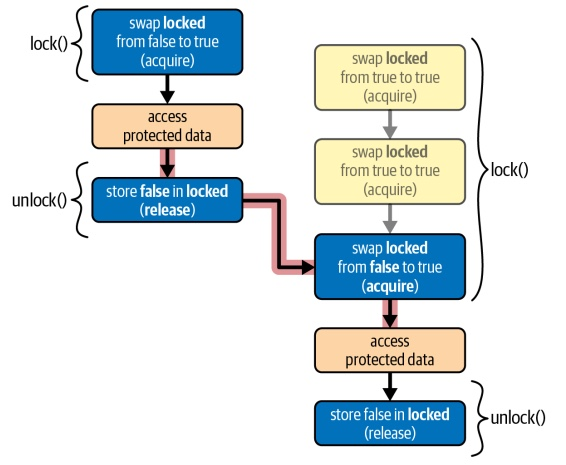
\includegraphics[width=.9\textwidth]{../images/ComputabilityAndRandomness/1.jpg}
\label{}
\end{figure}


\begin{corollary}[]
\(A\) is \(\Delta_2^0\) \(\Leftrightarrow\) \(A\) is both \(\Sigma_2^0\) and \(\Pi_2^0\)
\end{corollary}

\begin{proof}
\begin{align*}
A\in\Delta_2^0&\Leftrightarrow A\le_T\emptyset'\\
&\Leftrightarrow A\text{ and }\N-A\text{ are c.e. in }\emptyset'\\
&\Leftrightarrow A\in\Sigma_2^0\cap\Pi_2^0
\end{align*}
last iff from Theorem \ref{1.4.13}
\end{proof}


\begin{definition}[]
Let \(A\subseteq\N\) and \(n\ge 1\)
\begin{enumerate}
\item \(A\) is \(\Sigma_n^0\)if \(x\in A\leftrightarrow\exists y_1\forall y_2\dots Qy_nR(x,y_1,\dots,y_n)\), where \(R\) is a symbol for a
computable relation
\item \(A\) is \(\Pi_n^0\) if \(\N-A\) is \(\Sigma_n^0\)
\item \(A\) is \textbf{arithmetical} if \(A\) is \(\Sigma_n^0\) for some \(n\)
\end{enumerate}
\end{definition}

\begin{fact}[]
\label{1.4.12}
\(A\) is \(\Sigma_1^0\Leftrightarrow A\) is c.e.. The equivalence is uniform
\end{fact}

\begin{proof}
\(\Rightarrow\): Suppose \(x\in A\leftrightarrow\exists y R(x,y)\) for computable \(R\). Let \(\Phi\) be the partial computable
function given by the Turing program that on input \(x\) looks for a witness \(y\)
s.t. \(R(x,y)\), and halts when such a witness is found. Then \(A=\dom(\Phi)\)

\(\Leftarrow\): Suppose \(A=\dom(\Phi)\) for a partial computable function \(\Phi\). Let \(R\) be the computable
relation given by \(R(x,s)\leftrightarrow\Phi(x)[s]\downarrow\). Then \(x\in A\leftrightarrow\exists sR(x,s)\), so \(A\) is \(\Sigma_1^0\)
\end{proof}

A \(\Sigma_n^0\) set \(C\) is \textbf{\(\Sigma_n^0\)-complete} if \(A\le_mC\) for each \(\Sigma_n^0\) set \(A\)

\begin{theorem}[]
\label{1.4.13}
Let \(n\ge 1\)
\begin{enumerate}
\item \(A\) is \(\Sigma_n^0\) \(\Leftrightarrow\) \(A\) is c.e. relative to \(\emptyset^{(n-1)}\)
\item \(\emptyset^{(n)}\) is \(\Sigma_n^0\)-complete
\end{enumerate}
\end{theorem}

\begin{proof}
Induction on \(n\).  \ref{1.4.12} and \ref{1.2.2}. Now let \(n>1\)
\begin{enumerate}
\item First suppose \(A\) is \(\Sigma_n^0\) for some computable relation \(R\). Then the set
\begin{equation*}
B=\{\la x,y_1\ra:\forall y_2\dots Qy_nR(x,y_1,\dots,y_n)\}
\end{equation*}
is \(\Pi_{n-1}^0\) and \(A\) is c.e. relative to \(B\). By (2) for \(n-1\) we
have \(B\le_m\N-\emptyset^{(n-1)}\). So \(A\) is c.e. relative to \(\emptyset^{(n-1)}\)

Now suppose \(A\) is c.e. relative to \(\emptyset^{(n-1)}\). Then there is a Turing functional \(\Phi\)
s.t. \(A=\dom(\Phi^{\emptyset^{(n-1)}})\). By the use principle
\begin{equation*}
x\in A\Leftrightarrow\exists\eta,s\ucorner{\Phi_s^\eta(x)\downarrow\wedge\forall i<\abs{\eta}\;\eta(i)=1\leftrightarrow i\in\emptyset^{(n-1)}}
\end{equation*}
The innermost part can be put into \(\Sigma_n^0\)-form, so \(A\) is \(\Sigma_n^0\).
\item Follows by Proposition \ref{1.2.11} where \(Y=\emptyset^{(n-1)}\)
\end{enumerate}
\end{proof}

\begin{proposition}[]
Let \(n\ge 1\). Then \(A\) is \(\Delta_n^0\Leftrightarrow A\le_T\emptyset^{(n-1)}\)
\end{proposition}

\begin{proof}
By Theorem \ref{1.4.13}, \(A\) is \(\Delta_n^0\) \(\Leftrightarrow\) \(A\) and \(\N-A\) are c.e. in \(\emptyset^{(n-1)}\). By
Proposition \ref{1.2.8}, this condition is equivalent to \(A\le_T\emptyset^{(n-1)}\)
\end{proof}

\begin{proposition}[]
\(Z\) is \(\Sigma_2^0\) \(\Leftrightarrow\) there is a computable sequence of strong indices \((Z_s)_{s\in\N}\)
s.t. \(Z_s\subseteq[0,s)\) and \(x\in Z\leftrightarrow\exists s\forall t\ge s\;Z_t(x)=1\). The equivalence is uniform
\end{proposition}

\begin{proof}
\(\Rightarrow\): By Theorem \ref{1.4.13}, there is a Turing functional \(\Phi\) s.t. \(Z=\dom(\Phi^{\emptyset'})\). Now
let \(Z_s=\{x<s:\Phi^{\emptyset'}(x)[s]\downarrow\}\)

\(\Leftarrow\):
\end{proof}

\begin{definition}[]
The \textbf{index set} of a class \(S\) of c.e. sets is the set \(\{i:W_i\in S\}\)
\end{definition}


\begin{exercise}
\label{1.4.19}
\(\emptyset'\) is not an index set
\end{exercise}

\begin{proof}
We can find \(g\) s.t. \(W_{g(n)}=\{n\}\). Thus there is \(e\) s.t. \(W_{g(e)}=W_e=\{e\}\). By
padding lemma, we have \(W_i=W_e\) but \(i\notin\emptyset'\)
\end{proof}



\begin{exercise}
\label{1.4.20}
\begin{enumerate}
\item \(\{e:W_e\neq\emptyset\}\) is \(\Sigma_1^0\)-complete
\item The set \(\{e:W_e\text{ finite }\}\) is \(\Sigma_2^0\)-complete.
\item The set \(\Tot=\{e:\dom(\Phi_e)=\N\}=\{e:W_e=\N\}\) is \(\Pi_2^0\)-complete
\item Both \(\{e:W_e\text{ cofinite}\}\) and \(\Cop=\{e:W_e\text{ computable}\}\) are \(\Sigma_3^0\)-complete
\end{enumerate}
\end{exercise}

\begin{proof}
\begin{enumerate}
\item Given \(e\), \(\Phi_{f(n)}\) doesn't converge in \(\N-\{e\}\). And converges on \(e\)
if \(\Phi_e(e)\downarrow\). Thus \(\emptyset'\le_m\{e:W_e\neq\emptyset\}\)
\item Let \(\Fin=\{e:W_e\text{ finite}\}\). Then \(e\in\Fin\Leftrightarrow\exists s\forall t\ge s(W_{e,s}=W_{e,t})\)
\item \(e\in\Tot\Leftrightarrow\forall n\exists s\Phi_{e,s}(n)\downarrow\)

For any \(A\) in \(\Pi_2^0\), \(x\in A\Leftrightarrow\forall y\exists zR(x,y,z)\)

We could define
\begin{equation*}
\Phi_{q(x)}(u)=
\begin{cases}
0&\forall y\le u\exists zR(x,y,z)\\
\uparrow
\end{cases}
\end{equation*}
Then \(x\in A\Leftrightarrow W_{q(x)}=\omega\Leftrightarrow q(x)\in\Tot\)

\(x\in\barA\Leftrightarrow W_{q(x)}\) is finite
\item \(e\in\Cof\Leftrightarrow\exists z\forall n\ge z\exists s\Phi_{e,s}(n)\downarrow\), thus \(\Cof\in\Sigma_3^0\)

check fudan's textbook p120
\end{enumerate}
\end{proof}

\begin{exercise}
\label{1.4.21}
The set \(\{e:\dom\Phi_e^{\emptyset'}=\N\}\) is \(\Pi_0^3\)-complete
\end{exercise}

\begin{exercise}
\label{1.4.22}
Let \(\cals\) be a class of c.e. sets [\(\omega\)-c.e. sets] containing all the finite sets. Suppose the
index set of \(S\) is \(\Sigma_3^0\).  Then \(\cals\) is uniformly c.e. [uniformly c.e.]
\end{exercise}

\begin{proof}
Let \(I=\{e\mid\exists x\forall y\exists z\;R(e,x,y,.z)\}\), \(\cals=\{W_e\}_{e\in I}\)

\(\cals\) is \(\Sigma_3^0\), \(\cals\le_m\Cof\)
\end{proof}

\begin{exercise}
\label{1.4.24}
Let \(X\subseteq\N\)
\begin{enumerate}
\item Each relation \(R\le_TX\) is first-order definable in the structure \((\N,+,\cdot ,X)\)
\item The index set \(\{e:W_e\le_TX\}\) is \(\Sigma_3^0(X)\)
\end{enumerate}
\end{exercise}

\begin{proof}

\end{proof}

\begin{exercise}
\label{1.4.25}
\(A\) is \(\Delta_n^0\) \(\Leftrightarrow\) \(\forall x A(x)=\lim_{k_1}\dots\lim_{k_{n-1}}g(x,k_1,\dots,k_{n-1})\) for some
computable \(\{0,1\}\)-valued function \(g\)
\end{exercise}
\subsection{Absolute computational complexity of sets}
\label{sec:org6eb2f8c}
\subsubsection{Sets that are \texorpdfstring{\(low_n\)}{lown}}
\label{sec:orgdc0ef95}
\begin{definition}[]
Let \(f,g:\N\to\R\). \(f\) \textbf{dominates} \(g\) if \(f(n)\ge g(n)\) for almost every \(n\)
\end{definition}

\begin{enumerate}
\item \(A\) is \textbf{low} if \(A'\le_T\emptyset'\)
\item \(A\) is \textbf{computably dominated} if each function \(g\le_TA\) is dominated by a computable
function
\item \(A\) is \textbf{high} if \(\emptyset''\le_TA'\)
\end{enumerate}


\begin{definition}[]
Let \(n\ge 0\). We say that \(C\) is \(low_n\) if \(C^{(n)}\equiv_T\emptyset^{(n)}\)
\end{definition}

If \(C\in low_1\) we simply say that \(C\) is \textbf{low}. Each low set is \(\Delta_2^0\).

Each class \(low_n\) is closed downward under Turing reducibility, and contained in \(\Delta_{n+1}^0\)
\begin{equation*}
\text{computable}\subset low_1\subset low_2\subset\dots\subset\{Z:Z\not\ge_T\emptyset'\}
\end{equation*}

\begin{definition}[]
\(C\) is \textbf{superlow} if \(C'\equiv_{tt}\emptyset'\)
\end{definition}

It suffices to require that \(C'\le_{tt}\emptyset'\), because \(\emptyset'\le_mC'\) for any \(C\) by \ref{1.2.14}. By
\ref{1.4.4} it is equivalent to ask that \(C'\) be \(\omega\)-c.e.

\begin{definition}[]
\(A\) is \textbf{generalized \(low_1\)}, or in \(\GL_1\) for short, if \(A'\equiv_TA\oplus\emptyset'\)
\end{definition}

\begin{exercise}
\label{1.5.5}
If \(C\) is superlow, there is a computable function \(h\) s.t. \(Y\le_TC\) implies \(Y\le_{tt}\emptyset'\)
with use function bounded by \(h\) for each \(Y\)
\end{exercise}

\begin{proof}

\end{proof}

\begin{exercise}
\label{1.5.7}
If \(B\) is \(low_2\) then the index set \(\{e:W_e\le_TB\}\) is \(\Sigma_3^0\)
\end{exercise}

\begin{exercise}
\label{1.5.8}
\(B\) is \(low_2 \Leftrightarrow\) \(\Tot^B=\{e:\Phi_e^B\text{ total}\}\) is \(\Sigma_3^0\)
\end{exercise}
\subsubsection{Computably dominated sets}
\label{sec:orge219fd4}
\begin{definition}[]
\(A\) is called \textbf{computably dominated} if each function \(g\le_TA\) is dominated by a computable
function
\end{definition}

\(E\subseteq\N\)  is \textbf{hyperimmune} if \(E\) is infinite and \(p_E\) is not dominated by a computable
function, where \(p_E\) is the listing of \(E\) in order of magnitude

\begin{proposition}[]
\(A\) is not computably dominated \(\Leftrightarrow\) there is a hyperimmune set \(E\equiv_TA\)
\end{proposition}

\begin{proof}
\(\Leftarrow\): immediate since \(p_E\le_TE\)

\(\Rightarrow\): Suppose \(g\le_TA\) is not dominated by a computable function. Let \(E=\ran(h)\), where the
function \(h\) is defined as follows: \(h(0)=0\), and for each \(n\in\N\), \(h(2n+1)=h(2n)+g(n)+1\)
and \(h(2n+2)=h(2n+1)+p_A(n)+1\).
\end{proof}

\begin{proposition}[]
\(A\) is computably dominated \(\Leftrightarrow\) for each function \(f\)
\begin{equation*}
f\le_TA\to f\le_{tt}A
\end{equation*}
\end{proposition}

\begin{proof}
\(\Rightarrow\): Suppose \(f=\Phi^A\). Let \(g(x)=\mu s\Phi_s^A(x)\downarrow\). Then \(g\le_TA\), so there is a computable
function \(t\) s.t. \(t(x)\ge g(x)\) for each \(x\). Thus \(t\) bounds the running time of \(\Phi^A\),
whence \(f\le_{tt}A\) by Proposition \ref{1.2.22}
\end{proof}

\begin{proposition}[]
If \(A\) is \(\Delta_2^0\) and incomputable, then \(A\) is not computably dominated
\end{proposition}

\begin{proof}
Let \((A_s)_{s\in\N}\) be a computable approximation of \(A\). Then the following function \(g\) is
total
\begin{equation*}
g(s)\simeq\mu t\ge s.A_t\uhr s=A\uhr s
\end{equation*}
Note that \(g\le_TA\). Assume that there is a computable function \(f\) s.t. \(g(s)\le f(s)\) for
each \(s\). Then \(A\) is computable: for each \(n\) and each \(s>n\) we have \(A_t(n)=A(n)\)
for some \(t\in[s,f(s))\), namely \(t=g(s)\). On the other hand, if \(s\) is sufficiently large
then \(A_u(n)=A_s(n)\) for all \(u\ge s\). Thus to compute \(A\), on input \(n\) determine the
least \(s>n\) s.t. \(A_u(n)=A_s(n)\) for all \(u\in[s,f(s))\). Then \(A_s(n)=A(n)\), so the
output \(A_s(n)\) is correct
\end{proof}
\subsubsection{Sets that are \texorpdfstring{\(high_n\)}{highn}}
\label{sec:org2c27c16}
\begin{definition}[]
Let \(n\ge 0\). A set \(C\) is \(high_n\) if \(\emptyset^{(n+1)}\le_TC^{(n)}\)
\end{definition}

All the classes \(high_n\) are closed upward under Turing reducibility, so the complementary
classes \(\non-high_n=2^{\N}-high_n\) are closed downward. Therefore
\begin{equation*}
comp.\subset low_1\subset low_2\subset\dots\subset\non-high_2\subset\non-high_1\subset\{Z:Z\not\ge_T\emptyset'\}
\end{equation*}

It is easy to define a function \(f\le_T\emptyset'\) that dominates all computable functions: the
set \(\{\la e,x\ra:\Phi_e(x)\downarrow\}\) is c.e., and hence many-one reducible to \(\emptyset'\) via a computable
function \(h\). Let \(f(x)=\max\{\Phi_e(x):e\le x\wedge h(\la e,x\ra)\in\emptyset')\}\). If \(\Phi_e\) is total
then \(f(x)\ge\Phi_e(x)\) for all \(x\ge e\). This property of \(\emptyset'\) in fact characterizes the high
sets.

\begin{theorem}[]
\(C\) is high \(\Leftrightarrow\) some function \(f\le_TC\) dominates all computable functions
\end{theorem}

\begin{proof}
\(\Rightarrow\): We define a function \(f\le_TC\) that dominates each total \(\Phi_e\), extending the argument
for the case \(C=\emptyset'\). Note that \(\Tot=\{e:\Phi_e\text{ total}\}\) is \(\Pi_2^0\), and
hence \(\ove{\Tot}\le_m\emptyset''\le_TC'\). By the Limit Lemma \ref{1.4.2}, \(\Tot\) is \(\Delta_2^0(C)\), there is
a binary function \(p\le_TC\) s.t. for each \(e\), \(\lim_sp(e,s)\) exists and \(\lim_sp(e,s)=1\)
iff \(\Phi_e\) is total
\end{proof}
\end{document}
